
%%%%%%%%%%%%%%%%%%%%%%%%%%%%%%%%%%%%%%%%%%%%%%%%%%%%%%%%%%%%%%%%%%%%%%%
%                            Third Chapter                            %
%               Optimization on non-Euclidean Manifolds               %
%%%%%%%%%%%%%%%%%%%%%%%%%%%%%%%%%%%%%%%%%%%%%%%%%%%%%%%%%%%%%%%%%%%%%%%

\chapter{Optimization on non-Euclidean Manifolds}
\label{chapter:optimization_on_noneuclidean_manifolds}

\graphicspath{{Chapter4-Manifolds/Figs/}{Chapter4-Manifolds/Figs/Humanoids2015/}}

%{{{ LIST OF CONTRIBUTIONS
%\section{List of contributions}
%\begin{itemize}
  %\item{Optimization on Manifolds}
    %\begin{itemize}
      %\item Definition and examples of non-Euclidean manifolds
        %\begin{itemize}
          %\item $\mathbb{R}^n$
          %\item $SO(3)$
          %\item $S^2$
          %\item Cartesian Products
        %\end{itemize}
      %\item Representation space vs Tangent space vs manifold
      %\item Local parametrization, notion of retractation
      %\item Computation of function's derivatives, differentiation of retractation
      %\item Hessian update on manifolds, notion of vector transport and application to BFGS and SR1 updates
      %\item Computation of distances, notion of logarithm
    %\end{itemize}
  %\item{Practical Implementation: {\tt PGSolver}}
    %\begin{itemize}
      %\item General SQP algorithm adapted to local parametrization of manifolds.
      %\item Local QP and resolution with {\tt LSSOL}
      %\item Feasibility problems and resolution with {\tt LSSOL}
      %\item Acceptance criterion:
        %\begin{itemize}
          %\item Merit function
          %\item Filter
        %\end{itemize}
      %\item Globalization method:
        %\begin{itemize}
          %\item Line-Search
          %\item Trust-Region
            %\begin{itemize}
              %\item Notions of limit-Map vs trust-region vs problem's boundaries
              %\item Decisions of increase or decrease of trust region's size
              %\item Anisotrope trust-region
            %\end{itemize}
        %\end{itemize}
      %\item Hessian Update:
        %\begin{itemize}
          %\item BFGS
          %\item SR1
          %\item Fletcher LQNU
          %\item Individual vs grouped updates
          %\item Limited memory updates
        %\end{itemize}
      %\item Termination conditions:
        %\begin{itemize}
          %\item Satisfaction of KKT constraints
          %\item Null step
          %\item Failure of QP, FP, other\dots
        %\end{itemize}
      %\item Restoration Phase:
        %\begin{itemize}
          %\item Problem to solve: minimization of violation, relaxation of violated cstr
          %\item Exit condition: Feasible problem
          %\item Second-order correction phase
        %\end{itemize}
    %\end{itemize}
  %\item{Applications and testings of {\tt PGSolver} on non-robotic problems}
    %\begin{itemize}
      %\item Point cloud fitting
      %\item Surface parametrisation
      %\item Cube stacks
      %\item Schitkowsky
    %\end{itemize}
%\end{itemize}
%}}}

%{{{ INTRODUCTION TO OPTIMIZATION ON MANIFOLDS
\section{Introduction to optimization on Manifolds}
\label{sec:introduction_to_optimization_on_manifolds}

Posture generation has been traditionally formulated as a problem over a Euclidean space.
Robot variables may, however, be more naturally expressed over non-Euclidean manifolds.
The archetypes for this in robotics are the rotational part of the root body of a robot, and ball joints, whose variables live in $SO(3)$.
Some typical tasks are also naturally formulated on different manifolds.
For example, for making contact with any object that can be mapped on a sphere, the contact point position for this object can be parametrized in $S^2$~\cite{escande:icra:2016}.
The human shoulder can be elegantly parametrized on $S^2\times\mathbb{R}$, as proposed in~\cite{baerlocher}.
A non-Euclidean manifold can be thought of as a space that is locally Euclidean, but not globally.
Like a sphere, if one looks in a small enough neighborhood, it looks Euclidean, just like the surface of a giant sphere like the earth looks flat for a human standing on it.

Formulating the problem over $\mathbb{R}^n$ leads either to singularities that can prevent the convergence of the optimization solver, or cumbersome writing of additional constraints to specify that the variable is actually living on a manifold (see~\cite{bouyarmane:humanoids:2012}).
In addition, since constraints can be violated during the optimization process, the iterates may not be elements of the search manifold.

For example, let us consider an optimization problem over the $SO(3)$ manifold:

\begin{align}
\label{eq:pb_on_SO3}
  \minimize_{x \in SO(3)} & \quad f(x)\\
  \text{subject to}&
  \begin{array}{lr}
    l \leq c(x) \leq u \nonumber
  \end{array}
\end{align}

$SO(3)$ is a 3-dimensional manifold.
As such, it can be parametrized \emph{locally} by $3$ variables, for example, a choice of Euler angles.
But any such parametrization necessarily exhibits singularities when taken as a global map (e.g.\ gimbal lock for Euler angles), which can be detrimental to the optimization process.

For this reason, when addressing $SO(3)$ with classical optimization algorithms, it is often preferred to use one of the two following parametrizations:
\begin{itemize}
    \item unit quaternion, \emph{i.e.} an element $q$ of $\mathbb{R}^4$ with the additional constraint $\left\|q\right\| = 1$,
    \item rotation matrix, \emph{i.e.} an element $R$ of $\mathbb{R}^{3 \times 3}$ (or equivalently $\mathbb{R}^9$) with the additional constraints $R^T R = I$ and $\det{R} \geq 0$.
\end{itemize}

Then, if we use the unit quaternion parametrization, the problem~\Eqref{eq:pb_on_SO3} becomes:
\begin{align}
\label{eq:pb_on_SO3_quaternion}
  \minimize_{q \in \mathbb{R}^4} & \quad f(q)\\
  \text{subject to}&
  \left\{\begin{array}{lr}
    {l} \leq c(q) \leq {u} \nonumber\\
    {\|q\|}^2 - 1 = 0
  \end{array}\right.
\end{align}

The problem has 4 dimensions (to represent a 3-dimensional manifold), and has an additional constraint that is entirely due to our formulation choice.
With this formulation, it is guaranteed that the solution $q^*$ is a unit quaternion, but not that all the iterates $q_k$ along the optimization process have a unit norm.
During the optimization process, at each iteration, an increment $\mathbf{p}$ is computed by solving a quadratic problem that approximates~\Eqref{eq:pb_on_SO3_quaternion} locally around $q_k$.
In particular, this quadratic problem approximates the constraints linearly, thus, for any step $\mathbf{p}$ not null, even if iterate $q_k$ is of unit norm, the next iterate $q_{k+1} = q_k + \mathbf{p}$ does not respect the unit-norm constraint (it respects the \emph{linearization} of the unit-norm constraint).
So the quaternion $q_{k+1}$ does not represent a rotation, while the objective and constraints functions might expect it to do so.
%With non-manifold formulations, at any given iteration, the parametrization-related constraints can be violated, thus, the variables might not lie in the manifold.
In general, with non-manifold formulations, at any given iteration, the parametrization-related constraints can be violated, thus, the iterate might not lie in the manifold.
%Some additional treatment needs to be implemented.
It is then needed to project them on it.
%For example, all the functions involved in the problem can be composed with a normalization of the quaternion.
%Which in turn must be taken into account in the constraints and cost functions differentiations, which is an additional programming burden.
Denoting $\pi_\mathcal{M}$ the projection (for example $\pi_\mathcal{M} = \frac{q}{\left\|q\right\|}$ in the unit quaternion formulation), to evaluate a function $f$ on a manifold, we need to compute $f \circ \pi_\mathcal{M}$.
Furthermore, if the gradient is needed, then the projection must also be accounted for in its formulation (authors in~\cite{bouyarmane:humanoids:2012} explained this issue in great details for robotics problems with free-floating basis).

Similar issues can be found with the $\mathbb{R}^{3\times 3}$ matrix representation.

The alternative is to use optimization software working natively with manifolds, like the ones presented in~\cite{brossette:Humanoids:2015} or~\cite{absil:book:2008}, and solve the optimization problem as written in~\Eqref{eq:pb_on_SO3}.
This has an immediate advantage: we can write directly the problem without the need to add any parametrization-related constraints.
Working directly with manifolds also has the advantage that at each iteration, the variables of the problem represent an element of the manifold.
%This is not the case with the other formulations we discussed, as the (additional) constraints are guaranteed to be satisfied only at the end of the optimization process.
Having intermediate values naturally staying on the manifold can be useful to evaluate additional functions that pre-suppose it (additional constraints, external monitoring, etc.).
It can also be leveraged for real-time applications where only a short time is allocated repeatedly to the optimization, so that when the optimization process is stopped after a few iterations, the output is still meaningful in the sense that it is always a point of the manifold.

In this chapter, we present our nonlinear optimization solver able to work on generic smooth manifolds.
We take inspiration from the approach used for unconstrained optimization on manifolds in~\cite{absil:book:2008} and adapt it to constrained optimization.
To the best of our knowledge, studies on constrained optimization on manifolds have been few.
This is likely due to the fact that in most problems the only constraint is to be on the manifold.%, in that case, unconstrained optimization on manifold is enough.
We are only aware of the work of Schulman \emph{et al.}~\cite{Schulman2014}, where the authors explain the adaptation of their solver to work on $SE(3)$.
This adaptation is however not valid for general manifolds without more care for the Hessian computation.

A background motivation for this choice is to have our own optimization solver, instead of a black box.
This will allow us to specialize the solver for robotic problems, by leveraging modeling properties and approximations, for a gain in time and robustness.
%We also look forward to using this solver for problems with a varying number of constraints along the iterations (such as when complex collision constraints are considered).

%}}}
%{{{ OPTIMIZATION ON MANIFOLDS
\section{Optimization on Manifolds}
\label{sec:optimization_on_manifolds}

In this section, we describe a Sequential Quadratic Programming (SQP) approach~\cite{nocedal:book:2006} to solve the following nonlinear constrained optimization program

\begin{align}
\label{eq:optim_problem}
  \minimize_{x \in \mathcal{M}} & \quad f(x)\\
  \text{subject to}&
  \begin{array}{lr}
    l \leq c(x) \leq u \nonumber
  \end{array}
\end{align}

where $\mathcal{M}$ is a $n$-dimensional smooth manifold and $c$ is a $m$-dimensional real-valued function.
The inequality constraints can be replaced with an equality one when the upper and lower bounds are equal.

%{{{ REPRESENTATION PROBLEM
\subsection{Representation problem}
When $\mathcal{M} = \mathbb{R}^n$, the problem~\Eqref{eq:optim_problem} is solved iteratively, starting from an initial guess $x_0$ and performing successive steps $x_{i+1} = x_i + {\bf p_i}$ where ${\bf p_i}$ is the increment found at the $i$-th iteration, until convergence is achieved.
The strategy to compute ${\bf p_i}$ depends on the solver.

This classical scheme cannot be readily applied to optimization over non-Euclidean manifolds.
First of all, only (a subset of) the real numbers can be stored in computers.
To manipulate elements of $\mathcal{M}$ we need to choose a way to represent them in memory.
This results in choosing a representation space $\mathbb{E} = \mathbb{R}^r$ (with $r \geq n$) and a function
\begin{equation}
  \psi\ :\
  \begin{array}{ccc}
    x & \reduce{\mapsto}{6} & \mathbf{x} \\
    \mathcal{M} & \reduce{\rightarrow}{6} & \psi(\mathcal{M}) \subseteq \mathbb{E}
  \end{array}\nonumber%
\end{equation}
%In the following, we identify $\mathcal{M}$ with the set $\psi(\mathcal{M}) \subseteq \mathbb{E}$.
$\psi(\mathcal{M})$ is the subset of $\mathbb{E}$ containing the representation of all the elements of $\mathcal{M}$.
The projection operator $\pi_\mathcal{M}$ that we mentioned in Section~\ref{sec:introduction_to_optimization_on_manifolds} is actually a projection from $\mathbb{E}$ to $\psi(\mathcal{M})$.

With this representation, it is tempting to simply transform problem~\Eqref{eq:optim_problem} as an optimization over $\mathbb{R}^r$ with objective $f \circ \psi^{-1}$ and constraint $c \circ \psi^{-1}$, and solve it with a classical solver.
But, as we stated in Section~\ref{sec:introduction_to_optimization_on_manifolds}, if $r=n$ we get singularities, and if $r>n$ we add parametrization-related variables and constraints to our problem and the iterates may not lie on the manifold and need to be projected on it.
So both those approaches are not satisfactory, and another one needs to be taken.
%But depending on the representation choice, one of the two following problems arises:\\
%(i) $r=n$, then it is not possible in the general non-Euclidean case to find $\psi$ without derivative discontinuities.
%This can lead to critical convergence problems, \\
%(ii) $r>n$, then most elements of $\mathbb{E}$ do not represent an element of $\mathcal{M}$ %($\psi(\mathcal{M})$ is a measure-zero subset of $\mathbb{E}$)
%and $\psi$ cannot be surjective.
%Constraints need to be added to force the solution on $\mathcal{M}$.
%As a result, the problem has more variables and constraints w.r.t (i).
%Moreover, the additional constraints are unlikely to be met along the iteration process (even if $x_i$ is an element of $\mathcal{M}$, $x_i+{\bf p_i}$ is likely not, as nothing enforces it).
%This means that in order to evaluate $f \circ \psi^{-1}$ and $c \circ \psi^{-1}$ at a given $x_i$, one has to project it on $\psi(\mathcal{M})$ first, effectively computing $f \circ \psi^{-1} \circ \pi$ and $c \circ \psi^{-1} \circ \pi$, where $\pi$ is the projection.
%The composition by $\pi$ is an additional burden in programming (see e.g.\ in~\cite{bouyarmane:humanoids:2012a}).
%Figure~\ref{fig:stepOnSphere} illustrates the difference between a step through $\varphi$ in optimization on manifolds and a step followed by a projection as is done in classical optimization.

%\begin{figure}[htpb]
  %\centering
  %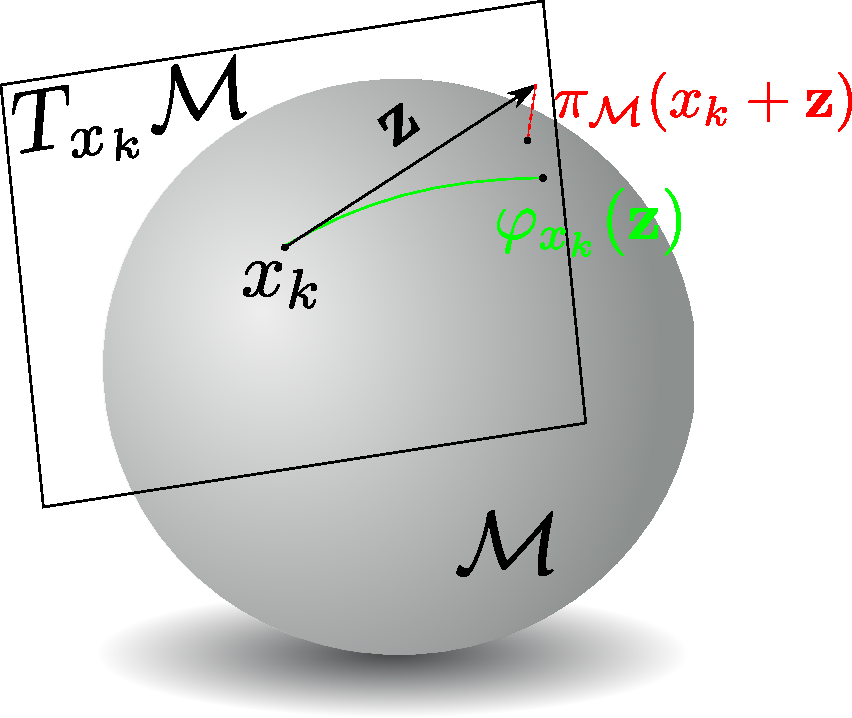
\includegraphics[width=0.5\linewidth]{Humanoids2015/stepOnSphere.pdf}
  %\caption{StepOnSphere}
%\label{fig:stepOnSphere}
%\end{figure}

%As a simple example, the set of 3D-rotations $SO(3)$ is a manifold of dimension $3$.
%The following (classical) choices can be made
%\begin{itemize}
  %\item Rotation matrix ${\bf R} \in \mathbb{R}^{3\times 3} \approx \mathbb{R}^9$, additional constraints: $\{{\bf R}^t{\bf R} = I\ ,\ \det({\bf R})=1\}$, projection by orthogonalization,
  %\item Quaternion ${\bf q} \in \mathbb{R}^4$, additional constraints: $\{ \left\|{\bf q}\right\|=1\}$, projection $\pi({\bf x}) = {\bf x}/\left\|{\bf x}\right\|$,
  %\item Euler angles ($\mathbb{E} = \mathbb{R}^3$), singularities when reaching gimbal lock.
%\end{itemize}

\begin{figure}[htpb]
  \centering
  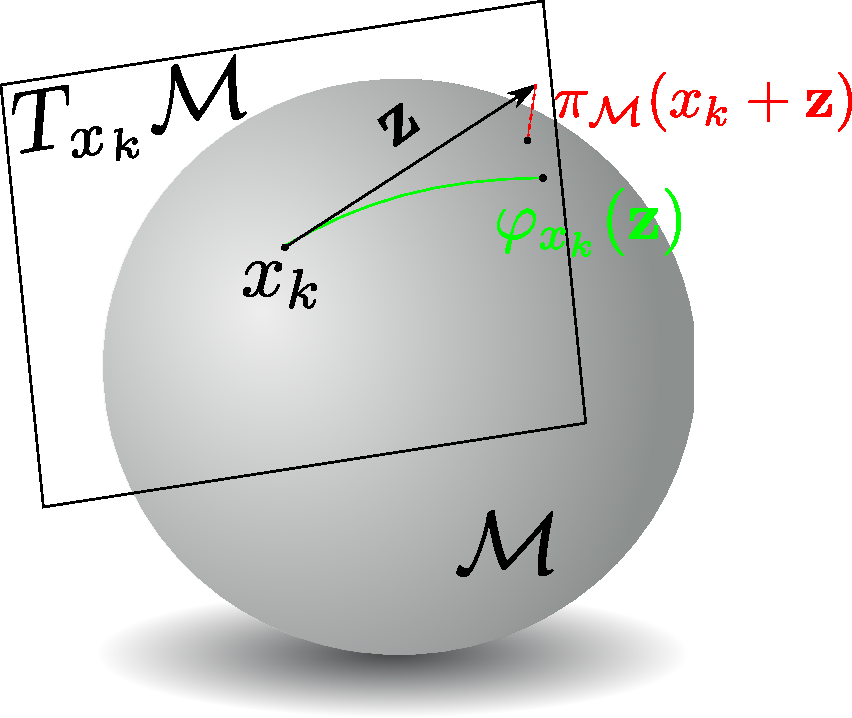
\includegraphics[width=0.5\linewidth]{Humanoids2015/stepOnSphere.pdf}
  \caption{StepOnSphere}
\label{fig:stepOnSphere}
\end{figure}


%}}}
%{{{ LOCAL PARAMETRIZATION
\subsection{Local parametrization}
By definition, there is always, at a point $x$ of a smooth $n$-dimensional manifold $\mathcal{M}$, a smooth function $\varphi_x$ between an open set of $T_x\mathcal{M}$, the tangent space to $\mathcal{M}$ at $x$ (which is isomorphic to $\mathbb{R}^n$), and a neighborhood of $x$ in $\mathcal{M}$, with $\varphi_x(0) = x$.

\begin{equation}
  \varphi_x\ :\
  \begin{array}{ccc}
    \mathbf{z} & \reduce{\mapsto}{6} & \varphi_x(\mathbf{z}) \\
    T_x\mathcal{M} & \reduce{\rightarrow}{6} & \mathcal{M}
  \end{array} \nonumber%
\end{equation}

$\varphi_x$ gives us a local parametrization for $\mathcal{M}$.
\Figref{fig:stepOnSphere} illustrates the difference between a step through $\varphi_x$ in optimization on manifolds and a step followed by a projection $\pi_\mathcal{M}$ as it can be done in classical optimization.

$T_x\mathcal{M}$ can be identified with $\mathbb{R}^n$, but in some cases, it needs to be considered as a hyperplane of a higher dimensionality space.
For example, in~\Figref{fig:stepOnSphere} and~\ref{fig:phimap}, $T_x\mathcal{M}$ is a 2-dimensional hyperplane embedded in $\mathbb{R}^3$.
We denote $T_x\mathbb{E}$ the representation space of $T_x\mathcal{M}$.
The driving idea of the optimization on manifolds is to change the parametrization of the problem by using a local function $\varphi_{x_i}$ at the current iterate $x_i$ at each iteration.
Applying this idea, we can reformulate Problem~\Eqref{eq:optim_problem} around $x_i$ as:
\begin{align}
\label{eq:local_problem}
\minimize_{{\bf z} \in T_{x_i}\mathcal{M}} & \quad f \circ \varphi_{x_i}({\bf z}) \\
  \text{subject to}&
  \begin{array}{rcl}
    {l} \leq & c \circ \varphi_{x_i}({\bf z}) & \leq {b} \nonumber
  \end{array}
\end{align}
This is an optimization problem on $\mathbb{R}^n$.
If we perform one iteration of a classical solver starting from $x_i$, we compute an increment ${\bf z_i}$, which leads to the next iterate $x_{i+1} = \varphi_{x_i}({\bf z_i})$.
We can then reformulate Problem~\Eqref{eq:optim_problem} around $x_{i+1}$, perform a new iteration and repeat the process until convergence.

\begin{figure}[!htb]
  \centering
  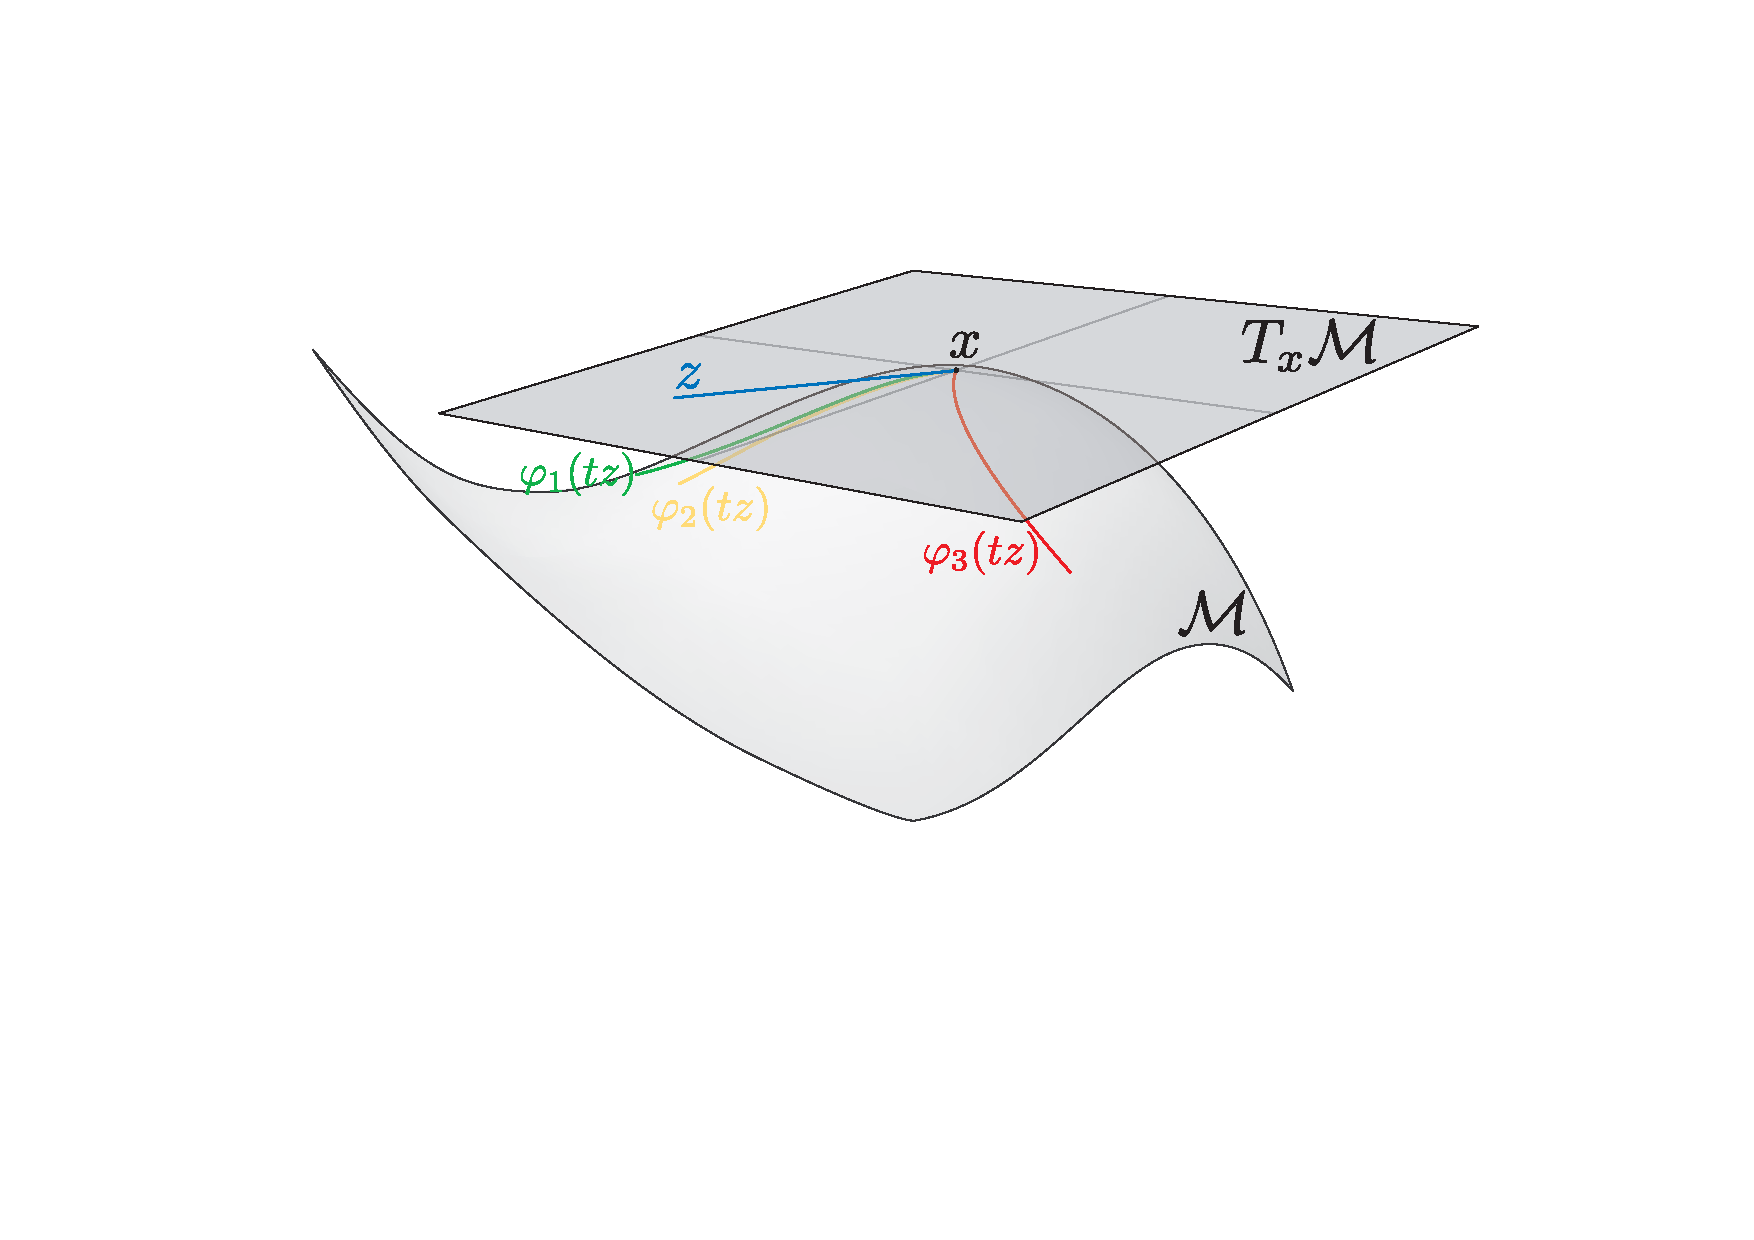
\includegraphics[width=.9\linewidth]{Humanoids2015/manifold.pdf}
  \caption{There are many possible choices for $\varphi_{x}$ but not all yield a curve $\varphi_{x}(t{\bf z})$ which is going in the same direction as ${\bf z}$: $\varphi_{1}$ and $\varphi_{2}$ are correct choices, $\varphi_{3}$ is not.}
\label{fig:phimap}
\end{figure}

However, convergence cannot be achieved without care on the choice of $\varphi_{x_i}$.
Once the optimization algorithm chooses an increment ${\bf z}_i$, we want to move from $x_i$ in the direction of ${\bf z}_i$ on the manifold.
In Euclidean spaces ($\mathbb{R}^n$), moving in the direction of a vector is straightforward.
On a manifold, the notion of moving in the direction of a tangent vector, while staying on the manifold, is generalized by the notion of retractation function.

A retractation $R$ at $x$, denoted $R_x$ is a function from $T_x{\mathcal{M}}$ to $\mathcal{M}$ with a local rigidity condition that preserves gradients at $x$.
Absil~\cite{absil:book:2008} defines a retractation as follows:
\begin{definition}
A retractation on a manifold $\mathcal{M}$ is a smooth function $R$ from the tangent bundle $T\mathcal{M}$ onto $\mathcal{M}$ with the following properties.
Let $R_x$ denote the restriction of $R$ to $T_x\mathcal{M}$.
\begin{enumerate}
  \item $R_x(0_x) = x$, where $0_x$ denotes the zero element of $T_x\mathcal{M}$.
  \item With the canonical identification $T_{0_x}T_x\mathcal{M}\approx T_x\mathcal{M}$, $R_x$ satisfies
  \begin{equation}
    DR_x(0_x) = \mathbf{1}_{T_x\mathcal{M}}
  \end{equation}
  Where $DR_x(0_x)$ denotes the gradient of $R_x$ at $0_x$ and $\mathbf{1}_{T_x\mathcal{M}}$ denotes the identity function on $T_x\mathcal{M}$.
\end{enumerate}
\end{definition}

This means that for any ${\bf z}$, the curve $t \mapsto \varphi_{x_i}(t{\bf z})$ is tangent to ${\bf z}$, see~\Figref{fig:phimap}, so that the update $x_{i+1} = \varphi_{x_i}({\bf z_i})$ is made in the direction given by ${\bf z_i}$.

The exponential map is a good theoretical candidate, but it is often impractical or expensive to compute.
Depending on the manifold, cheaper functions can be chosen such that $\varphi$ is a retractation.

With the iterative formulation approach described above, we do not have any parametrization issue, do not need additional constraints, and have the minimum number of optimization parameters.
We can use the function $\psi:\mathcal{M} \rightarrow \psi(\mathcal{M})$, which is surjective, to represent the $x_i$ and keep track of them in a global way.
%But we still need a map $\psi$ and real space $\mathbb{E}$ to represent the $x_i$ and keep track of them in a global way.
%The ${\bf x_i}$ are guaranteed to be on $\mathcal{M}$ so we can choose a representation with $r>n$ where $\psi$ is singularity-free without any drawback.
Also, the programmer can write the function $f' = f \circ \psi^{-1}$ as if it were a function from $\mathbb{E}$ to $\mathbb{R}$ without the need to project on $\psi(\mathcal{M})$ first (same goes for $c' = c \circ \psi^{-1}$).
For example, if $\mathcal{M} = SO(3)$ and $\mathbb{E} = \mathbb{R}^{3\times 3}$, ${\bf x_i}=\psi(x_i)$ is always a rotation matrix and can be used directly as such when writing the function.

%}}}
%{{{ LOCAL SQP ON MANIFOLDS
\subsection{Local SQP on manifolds}
\label{local_sqp_on_manifolds}

\begin{figure}[htpb]
  \centering
  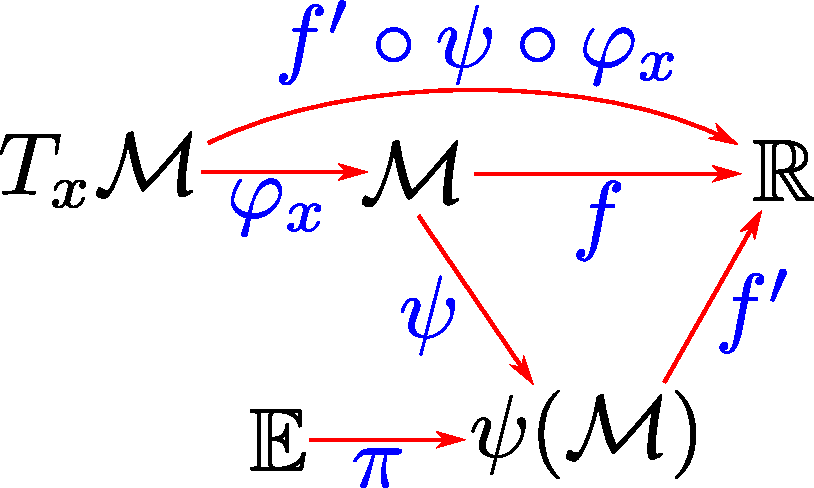
\includegraphics[width=0.5\linewidth]{diagramFunction.pdf}
  \caption{Diagram summarizing the different functions (in blue) and spaces (in black) used to represent a function on a manifold.}
\label{fig:diagram_function}
\end{figure}

We choose to adopt an SQP approach to solve our problem.
We first define the Lagrangian function
\begin{equation}
  %\mathcal{L}_x ({\bf z}, \lambda) = f\circ \varphi_x({\bf z}) - \lambda^T c \circ \varphi_x({\bf z})
  \mathcal{L}_x ({\bf z}, \lambda) = f\circ \varphi_x({\bf z}) - {\lambda_u}^T (c \circ \varphi_x({\bf z}) - u) - {\lambda_l}^T (c \circ \varphi_x({\bf z}) - l)
\end{equation}
with $\lambda_l \in \mathbb{R}^m$ and $\lambda_u \in \mathbb{R}^m$ the vector of Lagrange multipliers respectively associated with the lower and upper bound constraints.
The values of a Lagrange multiplier translate the activity status of the constraint it is associated with (see~\ref{sub:convergence_criterion}).

We denote $H_k$ the Hessian matrix $\nabla_{zz}^2 \mathcal{L}_{x_k}$.
Taking ${\bf z_0} = 0$, the $k$-th SQP step for Problem~\Eqref{eq:local_problem} is computed by solving the following quadratic program:

\begin{align}
  \label{eq:SQPStep}
  \minimize_{\bf z \in \mathbb{R}^n } & \quad {\frac{\partial f\circ \varphi_{x_k}}{\partial {\bf z}}(0)}^T {\bf z } + \frac{1}{2} {\bf z }^T H_k{\bf z }\\
  \text{subject to}&
  \begin{array}{lr}
    \text{l} \leq c\circ \varphi_{x_k}(0) + \frac{\partial c\circ \varphi_{x_k}}{\partial {\bf z}}(0) {\bf z }\leq \text{u}\\
  \end{array} \nonumber%
\end{align}

The basic SQP approach adapted to manifolds can be summarized as follows
\begin{enumerate}
  \item set $k=0$ and $x_k$ to the initial value
  \item compute ${\bf z}$ from Problem~\Eqref{eq:SQPStep} for current $x_k$
  \item set $x_{k+1} = \varphi_{x_k}({\bf z})$ and $k=k+1$
  \item if convergence is not yet achieved go to step 2
\end{enumerate}

Computations of function values and derivatives are based on the fact that $f \circ \varphi = f' \circ \psi \circ \varphi$ (and same for $c$), and
\begin{align}
  f'\ :\
  \begin{array}{ccc}
    \mathbb{E} & \reduce{\rightarrow}{6} & \mathbb{R}
  \end{array} \nonumber\\
  \psi\circ\varphi:
  \begin{array}{ccc}
    T_x{\mathcal{M}} & \reduce{\rightarrow}{6} & \mathbb{E}
  \end{array} \nonumber%
\end{align}
are representable functions (whereas $f$, $\psi$ and $\varphi_x$ are not, due to the fact that they feature $\mathcal{M}$ as input or output).
The gradient of $f \circ \varphi_x$ is
\begin{align}
  \frac{\partial f\circ\varphi_x}{\partial {\bf z}}=
  \frac{\partial f'}{\partial y}(\psi\circ\varphi_x)\times
  \frac{\partial (\psi\circ\varphi_x)}{\partial {\bf z}}
\end{align}

$\frac{\partial f'}{\partial y}$ denotes the gradient of $f'$ with respect to an element of $\mathbb{E}$, which is the derivative that is usually computed for use in classical optimization schemes.

In~\Figref{fig:diagram_function}, we present a summary of the different functions used in our approach to represent functions on manifolds.

\subsection{Vector transport}
\label{sub:vector_transport}

Nonlinear optimization algorithms such as the SQP rely on the second order information on the problem that is contained in the Hessian.
The exact value the Hessian is not always available, or might be too expensive to compute.
In these cases, we approximate the second order derivative by comparing first order information (tangent vectors) taken on distinct points of the manifold.
Much like in the case of the retractation operation, comparing tangent vectors on a Euclidean space is straightforward, but not on a manifold.

Given $x_1\in\mathcal{M}$ and $\mathbf{z}\in T_{x_1}\mathcal{M}$, we denote $x_2=\varphi_{x_1}(\mathbf{z})$.
We consider two vectors $\mathbf{v}_1 \in T_{x_1}\mathcal{M}$ and $\mathbf{v}_2 \in T_{x_2}\mathcal{M}$ that we want to compare, it is necessary to transport $\mathbf{v}_1$ into $T_{x_2}\mathcal{M}$.

Absil~\cite{absil:book:2008} gives a formal definition of the vector transport in chapter 8.

One can describe the vector transport function from a point $x\in \mathcal{M}$ along an increment $\mathbf{z}$ as:
\begin{equation}
  \mathcal{T}_{x,z} :\
  \begin{array}{ccc}
    \mathbf{v} & \reduce{\mapsto}{6} & \mathcal{T}_{x,\mathbf{z}}(\mathbf{v}) \\
    T_x\mathcal{M} & \reduce{\rightarrow}{6} & T_{\varphi_x(\mathbf{z})}\mathcal{M}
  \end{array} \nonumber%
\end{equation}

%The vector transport can be defined as follows~\cite{absil:book:2008}.

%Let $T\mathcal{M}\oplusT\mathcal{M}=\{(\mathbf{z},\mathbf{v}):\mathbf{z}, \mathbf{v}\in T_x\mathcal{M}, x\in \mathcal{M}$
%\begin{definition}
  %A vector transport on a manifold $\mathcal{M}$ is a smooth mapping
  %\begin{equation}
    %T\mathcal{M}\oplus T\mathcal{M} \rightarrow T\mathcal{M}:(\mathbf{z},\mathbf{v})\mapsto \mathcal{T}_
  %\end{equation}
%\end{definition}

\Figref{fig:transport} illustrates the transport of a vector $\mathbf{v}_1$ from $T_{x_1}\mathcal{M}$ to $T_{x_2}\mathcal{M}$.
%$\mathbf{v}_2$ can then be compared to the transported $\mathbf{v}_1$: $\mathcal{T}_{x_1,\mathbf{z}}(\mathbf{v}_1)$.
%This operation will come in handy for the computation of Hessian approximations explained in Section~\ref{sub:hessian_update_on_manifolds}.

\begin{figure}[htpb]
  \centering
  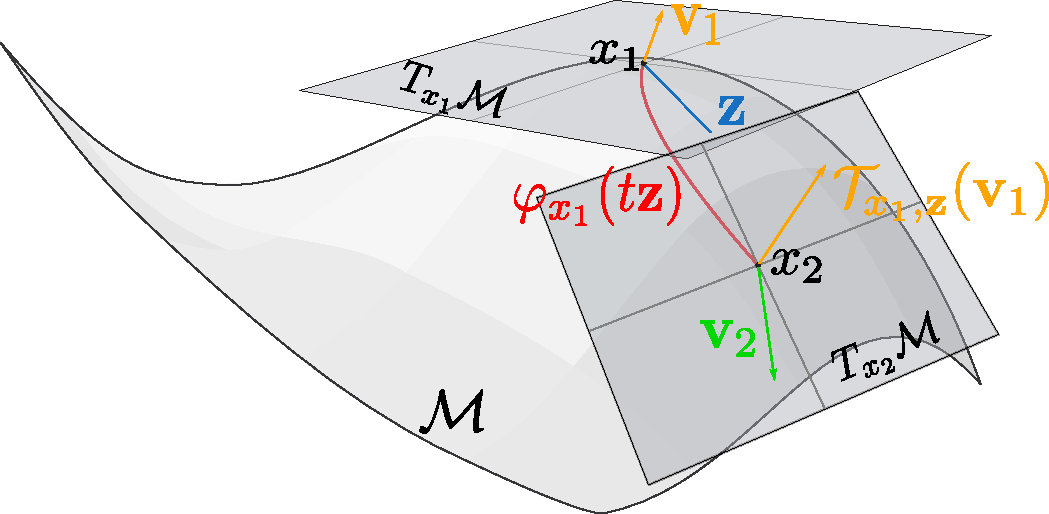
\includegraphics[width=0.8\linewidth]{transport.pdf}
  \caption{Vector transport on a non-Euclidean manifold.}
\label{fig:transport}
\end{figure}


%}}}
%{{{ DESCRIPTION OF NON-EUCLIDEAN MANIFOLDS
\subsection{Description of non-Euclidean manifolds}
\label{sub:examples_on_non_euclidean_manifolds}

In order to develop an optimization algorithm on manifolds, we need to define a set of elements and operations for each elementary manifold $\mathcal{M}$ that will enable us to handle its elements with ease.
%For each elementary manifold $\mathcal{M}$, we need to define a set of elements and operations.
They need to be implemented once only (it is then trivial to get those functions for Cartesian products of manifolds).
The composition with $f'$ and $c'$ is done automatically.
The expression of those functions is adapted from~\cite{boumal:jmlr:2014}.

\paragraph{Retractation:}
We need a retractation operator $\phi_x = \psi\circ\varphi_x$ and its derivative.
During the optimization process, we need the expression of the derivatives of $\phi_x$ in order to compute the gradients of the cost function and of the constraints at the beginning of each iteration.
Because we change the parametrization of our problem to be centered on $x_k$ at each iteration, we only need to evaluate the gradient of $\phi_x$ for $\mathbf{z}=0$, $\frac{\partial \phi_x}{\partial \mathbf{z}}(0)$.
In some cases, this quantity is invariant w.r.t $x$ and can be computed once and for all.

\paragraph{Pseudo-logarithm and distances:}
It is interesting to compute distances on manifolds.
For that, we define the pseudo-logarithm operator (denoted pseudolog), which is the inverse of the retractation operator.
\begin{equation*}
  \zeta_x:\mathcal{M}\rightarrow T_x\mathcal{M}
\end{equation*}
\begin{equation*}
  \forall (x,y)\in \mathcal{M}\times\mathcal{M},\ \mathbf{z}=\zeta_x(y)\ \text{is such that}\ \phi_x(\mathbf{z}) = y
\end{equation*}
The pseudolog operator computes the vector of $T_x\mathcal{M}$ to go from $x$ to $y$.
It is used to compute the (pseudo-) distance between two points of $\mathcal{M}$
\begin{equation*}
  \dist(x,y) = \|\zeta_x(y)\|
\end{equation*}

\paragraph{Vector transport:}
To compare two vectors living in the tangent spaces of different points of $\mathcal{M}$, it is necessary to use the vector transport operation to transport one of them in the space of the other one before comparing them, see~\Figref{fig:transport}.
%To compare two vectors of the tangent spaces of $\mathcal{M}$, it is necessary to use the vector transport operation to transport one of them in the space of the other one before comparing them, see Figure~\ref{fig:transport}.
%To compare two vectors $\mathbf{v}_1$ and $\mathbf{v}_2$ defined in tangent spaces of different points, respectively, $T_{x_1}\mathcal{M}$ and $T_{x_2}\mathcal{M}$, it is necessary to transport $\mathbf{v}_1$ into $T_{x_2}\mathcal{M}$.
%Figure~\ref{fig:transport} illustrates the transport of a vector $\mathbf{v}_1$ from $T_{x_1}\mathcal{M}$ to $T_{x_2}\mathcal{M}$.
%$\mathbf{v}_2$ can then be compared to the transported $\mathbf{v}_1$: $\mathcal{T}_{x_1,\mathbf{z}}(\mathbf{v}_1)$.
This operation will come in handy for the computation of Hessian approximations explained later in this chapter.


\paragraph{Projections:} It is useful to define a projection operator on $\mathcal{M}$, as well as one on $T_x\mathcal{M}$, especially to help eliminate some numerical errors when necessary.
The projection operator on $\mathcal{M}$ projects an element of $\mathbb{E}$ onto $\psi(M)\subseteq \mathbb{E}$ while the one on $T_x{M}$ projects an element of $\mathbb{E}$ onto $T_x\mathcal{M}$.

%\paragraph{Limits on tangent map:} The tangent map can present some singularities, thus it is necessary to limit the length of steps made through retractation to the validity region of each manifold.
\paragraph{Limits of validity of the retractation:} The retractation is only valid locally, and we need to give a (conservative) approximation of its validity region.

To summarize, for each elementary manifold $\mathcal{M}$, we need to implement the following elements:
\begin{itemize}
  \item Tangent space at point $x$, $T_x\mathcal{M}$
  \item Embedding spaces $\mathbb{E}$ and $T_x\mathbb{E}$
  \item Retractation operator $\phi:\ (x,\mathbf{z}) \rightarrow \phi_x(\mathbf{z})$
  \item Gradient of the retractation operator at zero $\partial \phi(x):\rightarrow \frac{\partial \phi_x}{\partial \mathbf{z}}(0)$
  \item Pseudo-logarithm operator $\zeta:\ (x,y) \rightarrow \zeta_x(y)$
  \item Gradient of pseudo-logarithm operator at the iterate $\frac{\partial \zeta_x}{\partial y}(x)$
  \item Transport operator $\mathcal{T}:\ (x,\mathbf{z}, \mathbf{v})\rightarrow \mathcal{T}_{x,\mathbf{z}}(v)$
  \item Projection from $\mathbb{E}$ on $\mathcal{M}$, $\pi_\mathcal{M}$
  \item Projection from $T_x\mathbb{E}$ on $T_x\mathcal{M}$, $\pi_{T_x\mathcal{M}}$
  \item Limits of validity of the retractation on $T_x\mathcal{M}$, $\lim$
\end{itemize}

We provide the detailed formulas for those operations in Appendix~\ref{appendix:manifolds} for different elementary manifolds:
\begin{itemize}
  \item The Real space of dimension $n$ in~\ref{sec:the_real_space}
  \item The 3D rotations manifold SO(3) with matrix formulation in~\ref{sec:the_3d_rotation_manifold_matrix_representation}
  \item The 3D rotations manifold SO(3) with quaternion formulation in~\ref{sec:the_3d_rotation_manifold_quaternion_representation}
  \item The unit sphere manifold $S^2$ in~\ref{sec:the_unit_sphere_manifold_s2}
\end{itemize}

%{{{ CARTESIAN PRODUCT OF MANIFOLDS
\subsubsection{Cartesian Product of Manifolds}
\label{ssub:cartesian_product_of_manifolds}
Given two manifolds $\mathcal{M}_1$ and $\mathcal{M}_2$, we denote $\mathcal{M}=\mathcal{M}_1\times\mathcal{M}_2$ their cartesian product.
Any operation on an element of $\mathcal{M}$ can simply be computed term by term for each manifold composing $\mathcal{M}$.
For example, the retractation is computed as follows, and that scheme can be reproduced for all other operations:

\begin{align}
  &x_1\in \mathcal{M}_1,\ \mathbf{z_1}\in T_{x_1}\mathcal{M}_1,\ x_2\in \mathcal{M}_2,\ \mathbf{z_2}\in T_{x_2}\mathcal{M}_2\\
  &x=\begin{bmatrix}
    x_1\\x_2\\
  \end{bmatrix}\in \mathcal{M},\ \mathbf{z}=\begin{bmatrix}
    \mathbf{z_1}\\ \mathbf{z_2}\\
  \end{bmatrix}\in T_x\mathcal{M}\\
  &\phi_x(z) = \begin{bmatrix}
    \phi_{x_1}(\mathbf{z_1})\\
    \phi_{x_2}(\mathbf{z_2})\\
  \end{bmatrix}
\end{align}

%}}}

\subsection{Implementation of Manifolds}
\label{sub:implementation_of_manifolds}

In order to use the manifold formulation described above in other software, and particularly in a numerical solver, we wrote an independent C++ project.
This implementation is open-source and available at \href{https://github.com/stanislas-brossette/manifolds}{https://github.com/stanislas-brossette/manifolds}.
The implementation consists of 3 types of classes: the Manifold class, the elementary manifold classes, and the Point class.
The Manifold class describes the abstract mathematical structure of a non-Euclidean manifold and defines a common interface for all elementary manifolds to implement (retractation, pseudoLog,\ldots).
Elementary Manifold classes ($\mathbb{R}^n$, $SO(3)$, $S^2$, and the Cartesian Product) are the concrete manifolds.
They inherit from the Manifold class and implement all their mathematical operations.
The Cartesian Product class is used to build compound manifolds by being `multiplied' with other elementary manifolds.
The Point class represents a point on a manifold, it contains the data that represents its numerical value.
It can only be constructed by a manifold, and provides some proxy to its manifolds operations.
In particular, it is equipped with an increment method, that applies a retractation on it.
\Figref{fig:uml_manifold} presents a simplified class diagram of this project, omitting all the settor, gettor, bookkeeping mechanics and accessory functions.

\begin{figure}[htpb]
  \centering
  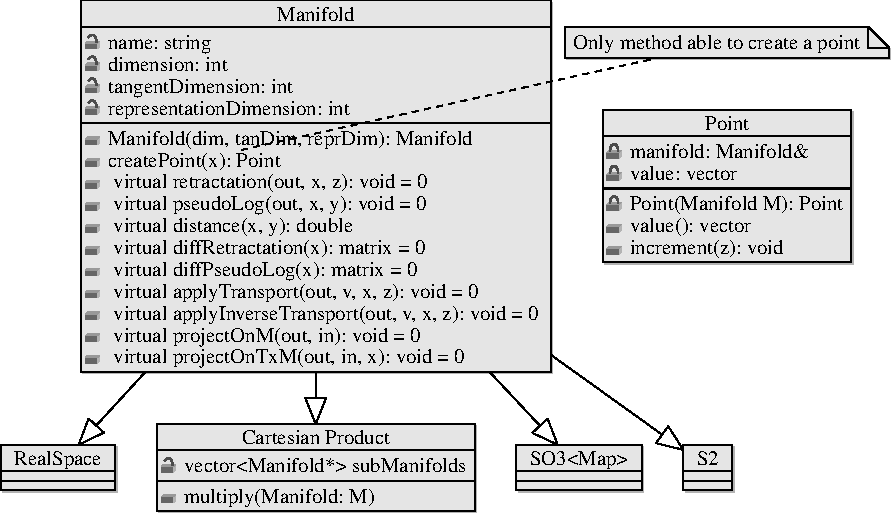
\includegraphics[width=\linewidth]{uml/manifolds-1.pdf}
  \caption{Simplified class diagram of the Manifold project.}
\label{fig:uml_manifold}
\end{figure}

%}}}
%{{{ PRACTICAL IMPLEMENTATION
\section{Practical implementation}
\label{sec:practical_implementation}

The SQP algorithm presented in Section~\ref{local_sqp_on_manifolds} works locally, \emph{i.e.} it is guaranteed to converge when starting close enough to the solution.
In practice, various refinements are made to ensure convergence from any starting point, it is called the globalization.
We detail hereafter the choices we made for the implementation of our solver called {\tt PGSolver}.

We summarize the entire SQP algorithm in Diagrams~\ref{fig:main_sqp_loop},~\ref{fig:restoration_loop} and~\ref{fig:second_order_correction}, which represent respectively the main SQP loop, the restoration phase, and the second order correction algorithm.

\subsection{Linear and quadratic problems resolution}
\label{sub:linear_and_quadratic_problems_resolution}

The central idea of an SQP algorithm is that it solves a series of QP iteratively until a solution is reached.
There are many off-the-shelf QP solvers available and the state of the art is mature in that field.
Thus, we decided to use the {\tt LSSOL} solver~\cite{gill:techrep:1986}.
{\tt LSSOL} provides resolution methods for several types of problems and we are interested in using the resolution methods for FP (Feasibility Problem) and QP.
The {\tt LSSOL} framework formulates problems as follows (Note that there are no equality constraints in this formulation):

\begin{align}
  \minimize_{x\in \mathbb{R}^n}\ &{F(x)}\\
  \text{subject to}\  & l\leq \begin{Bmatrix}
    x\\
    Cx
  \end{Bmatrix}
  \leq u
\end{align}

With the $F$ function taking different forms depending on the problem to solve:
\begin{table} [H]
\centering
\begin{tabular}{ccc}
  \toprule
  FP:\@ & None & (find a feasible point for the constraints)\\
  \midrule
  QP2: & $F(x)=c^T x+\frac{1}{2} x^T A x$ & $A$ symmetric and positive semi-definite \\
  \midrule
  QP4: & $F(x)=c^T x+\frac{1}{2} x^T B^T B x$ & $B$ $m\times n$ upper-trapezoidal \\
  \bottomrule
\end{tabular}
\end{table}

The QP4 type of problem is used when a decomposition of the matrix $A$ of QP2, $A=B^T B$ is already available.

\subsection{Problem Definition}
\label{sub:problem_definition}

As stated in Eq~\Eqref{eq:pb_on_SO3} we want to solve a nonlinear constrained optimization problem on manifold that takes the following form:

\begin{align}
  \minimize_{x \in \mathcal{M}} & \quad f(x)\\
  \text{subject to}&
  \begin{array}{lr}
    l \leq c(x) \leq u \nonumber
  \end{array}
\end{align}

The list of constraints can be separated into 3 categories: Bounds, Linear, and Nonlinear.
For convenience, we formulate our optimization problem in a way that is compatible with {\tt LSSOL} by changing all equality constraints into inequality constraints:

\begin{equation}
  c(x) = a \Leftrightarrow a \leq c(x) \leq a
\end{equation}

Our problem can be written as:
\begin{align}
\label{eq:optim_problem_on_manifold}
  \minimize_{x \in \mathcal{M}} & \quad f(x)\\ \nonumber
  \text{subject to}&\left\{
  \begin{array}{lr}
    L_B \leq x \leq U_B \\
    L_L \leq Ax \leq U_L \\
    L_N \leq c(x) \leq U_N
  \end{array}\right.
\end{align}

With $L_B$ and $U_B$ being respectively the lower and upper bounds for Bounds constraints, $L_L$ and $U_L$ the lower and upper bounds for Linear constraints, and $L_N$ and $U_N$ the lower and upper bounds for Nonlinear constraints.
That formulation is conveniently used to define our problem.
Since we are solving this problem on a non-Euclidean manifold, we need to re-formulate it around the current iterate $x_i$ at each iteration.
This is done automatically behind the scene and the user only has to provide the information to build problem~\Eqref{eq:optim_problem_on_manifold}.

At iteration $i$, the problem becomes (for clarity, we drop the subscript $i$ that goes with each appearance of $x$):
\begin{align}
\label{eq:optim_problem_on_txm}
  \minimize_{\mathbf{z} \in T_x\mathcal{M}} & \quad f(\phi_x(\mathbf{z}))\\ \nonumber
  \text{subject to}&\left\{
  \begin{array}{lr}
    {\bf z}_{\text{map}}^- \leq \mathbf{z} \leq {\bf z}_{\text{map}}^+ \\
    L_B \leq \phi_x(\mathbf{z}) \leq U_B \\
    L_L \leq A\phi_x(\mathbf{z}) \leq U_L \\
    L_N \leq c(\phi_x(\mathbf{z})) \leq U_N \\
  \end{array}\right.
\end{align}

With ${\bf z}_{\text{map}}^-$ and ${\bf z}_{\text{map}}^+$ being respectively the lower and upper bounds of validity of the tangent map of $\mathcal{M}$ around $x$.
After this reformulation, we note that if $\phi_x$ is nonlinear, then the bounds and linear constraints of problem~\Eqref{eq:optim_problem_on_manifold} become nonlinear in problem~\Eqref{eq:optim_problem_on_txm}.
It is then necessary to treat the problem and evaluate which constraint is linear and which is not, in order to go back to a formulation of the same type as in problem~\Eqref{eq:optim_problem_on_manifold}.
Basically, for each constraint $c_j$ in problem~\Eqref{eq:optim_problem_on_txm}, if the submanifold of $\mathcal{M}$ on which that constraint is applied is a real space $\mathbb{R}^m$ then the constraint maintains its bound, linearity or nonlinearity status, otherwise, it becomes a nonlinear constraint\footnote{This treatment of the constraints is a planned work, it has not been implemented yet.}.
It is, however, unusual to write linear constraints on non-Euclidean manifolds.
%Once again, this may look like a drawback of optimization on manifolds, but it is usually the same with classical optimization.
%Indeed, a linear constraint on the representation space of a non-Euclidean manifold might not often make much sense.
%For example, a linear constraint on the elements of a unit quaternion, although one can obviously be devised, does not seem to make much sense.
%So usually, when a non-Euclidean manifold is involved, the constraint is nonlinear.

In the particular case of linear constraints (and by extension bound constraints) on a submanifold that is a real space, the constraints on $x$ are transformed into constraints on $z$ as follows:
\begin{equation}
  L_L \leq Ax \leq U_L \ \Rightarrow \ L_L - Ax \leq A\mathbf{z} \leq U_L-Ax
\end{equation}
For bounds constraints, the same goes with $A$ being the identity matrix on the submanifold.

Once those substitutions are done, we obtain a new problem of the following form (where $L_B'$, $L_L'$, $L_N'$, $U_B'$, $U_L'$, $U_N'$ are the lower and upper bounds for the bounds, linear and nonlinear constraint, $A'$ is the matrix of linear constraints and $c'$ is the list of nonlinear functions):

\begin{align}
\label{eq:optim_txm_final}
  \minimize_{\mathbf{z} \in T_x\mathcal{M}} & \quad f \circ \phi_x(\mathbf{z})\\ \nonumber
  \text{subject to}&\left\{
  \begin{array}{lr}
    L_B' \leq \mathbf{z} \leq U_B' \\
    L_L' \leq A' \mathbf{z} \leq U_L' \\
    L_N' \leq c' \circ \phi_x(\mathbf{z}) \leq U_N'\\
  \end{array}\right.
\end{align}

This problem is an exact reformulation of problem~\Eqref{eq:optim_problem_on_manifold} on $T_x\mathcal{M}$.
At each step of the optimization process, we solve the QP approximating this problem~\Eqref{eq:optim_txm_final} around $\mathbf{z}=0$.
The Taylor development of $c\circ\phi_x(z)$ to the first order around $\mathbf{z} = 0$ gives:
\begin{equation}
  c' \circ \phi_x(\mathbf{z}) \approx c'\circ \phi_{x_k}(0) + \frac{\partial c'\circ \phi_{x_k}}{\partial {\bf z}}(0) {\bf z } = c'(x_k) + {\left(\nabla\phi_{x_k}(0) \nabla c' (x_k)\right)}^T\mathbf{z}
\end{equation}

The trust-region constraint (see Section~\ref{sub:trust_region_and_limit_map}) is added to the problem to limit the length of a step, $\rho$ denotes the size of the trust-region.
$H_k$ is an estimation of the Hessian computed as shown in Section~\ref{sub:hessian_update_on_manifolds}.
The QP to be solved at each iteration is the following:

\begin{align}
  \label{eq:QP_txm}
  \begin{split}
  \minimize_{\mathbf{z} \in T_x\mathcal{M}=\mathbb{R}^n } & \quad {\left(\nabla\phi_{x_k}(0) \nabla f (x_k)\right)}^T\mathbf{z} + \frac{1}{2} {\bf z }^T H_k{\bf z }\\
  \text{subject to}&\left\{
  \begin{array}{lr}
    L_B' \leq \mathbf{z} \leq U_B' \\
    L_L' \leq A' \mathbf{z} \leq U_L' \\
    L_N' \leq c'(x_k) + {\left(\nabla\phi_{x_k}(0) \nabla c' (x_k)\right)}^T\mathbf{z}\leq U_N'\\
    -\rho \leq \mathbf{z} \leq \rho \quad (\text{trust-region constraint}) \\
  \end{array}\right.
  \end{split}
\end{align}

The resolution of this QP~\Eqref{eq:QP_txm} (with {\tt LSSOL}) gives the optimal solution $\mathbf{z}^*$ and Lagrange multipliers $\lambda^*$.
The new iterate that will be considered is:
\begin{align}
  x_{k+1} & \leftarrow \phi_{x_k}(\mathbf{z}^*)\\
  \lambda_{k+1} & \leftarrow \lambda^*
\end{align}

Note that the only additional computation due to the formulation on manifolds is the multiplication of the gradients of constraints and cost by the map's gradient at $0$.
The computation time related to those products can be reduced by taking advantage of the fact that $\nabla \phi_x(0)$ is block-diagonal.

\subsection{Trust-region and limit map}
\label{sub:trust_region_and_limit_map}

Maps $\varphi_{x}$ are only valid locally, and we need to be aware of this fact: a step ${\bf z}$ found by solving Problem~\Eqref{eq:QP_txm} should not be outside the validity region of the map.
This can be enforced by adding the limits of the manifold map to the problem as bound constraints.
In fact, this can be done by intersecting the original problem's bounds with the limits of the map and imposing the resulting bounds as constraints.
This leads naturally to trust region methods that we, therefore, favor over line-search approaches.
We present the classical trust-region strategy in Section~\ref{ssub:the_trust_region_strategy}.

In the case of a robotics problem, different variables often have different orders of magnitude, for example, contact forces can be of the order of hundreds of Newtons, depending on the weight and torque capacity of the robot, while joint angles are of the order of radians.
Let $x$ be the variable vector of such problem with $x={[\theta_0, \theta_1, f_0, f_1, f_2]}^T$ where $\theta_i$ represent angular variables and $f_i$ forces.
The shape of the trust-region should reflect those differences, but we want to keep the simplicity of the classical trust-region strategy.
For that, we propose to separate the trust-region $\rho$ in two parts: its scale $\rho_\text{scale}$ which is a scalar, and its shape $\rho_\text{shape}$ which in a vector of dimension $n$ (that value is actually stored in the instance of manifold).
$\rho_\text{shape}$ is constant and set at the beginning of the optimization, the i-th element of $\rho_\text{shape}$ is the order of magnitude of the i-th dimension of the optimization variable.
In the previous example, we'd get ${\rho_\text{shape}} = {[1,1,100,100,100]}^T$
And $\rho_\text{scale}$ is the scalar that gets updated in the trust-region strategy.

Finally, the constraints related to the trust-region added to the problem is:
\begin{equation}
  -\rho = -\rho_\text{scale}\rho_\text{shape} \leq \mathbf{z} \leq \rho_\text{scale}\rho_\text{shape} = \rho
\end{equation}

\subsection{Filter method}
\label{sub:filter_method}

To know if a step ${\bf z}$ is acceptable or not, one usually uses a penalty-based merit function as we present in Section~\ref{sec:resolution_of_a_non_linear_constrained_optimization_problem}.
In our early tests, the update of the penalty parameters proved to be difficult with our types of problems.
We now use a filter approach instead, as presented in Section~\ref{ssub:the_filter_method}.

Our algorithm is an adaptation of Fletcher's filter SQP~\cite{fletcher:mathprog:2000} to the case of manifolds: we use an adaptive trust-region that is intersected with the validity region of $\phi_{x_i}$, and a new iterate $x_{i+1} = \phi_{x_i}({\bf z})$ is accepted if either the cost function or the sum of constraint violations is made better than for any previous iterates.

\subsection{Convergence criterion}
\label{sub:convergence_criterion}

An iterate $\{x,\lambda\}$ is considered to be a solution of the optimization problem if it satisfies the first-order optimality conditions (presented in Section~\ref{sub:optimality_conditions}) to within certain tolerances.
We use the same criterion as the one used in \href{http://www.sbsi-sol-optimize.com/asp/sol_product_snopt.htm}{{\tt SNOPT}} and presented in~\cite{gill:snopt:2002}.
It has the advantage of using two different tolerance constants: $\tau_P$ monitors the primal optimality conditions, which means the satisfaction of the constraints, and $\tau_D$ monitors the dual conditions, which means the optimality of the cost function and of the Lagrange multipliers.
That gives the user more control over the quality of the solution.

Dropping the distinction between Linear and Nonlinear Constraints,
the problem can be rewritten as:

\begin{align}
\begin{split}
\label{eq:problem}
  \minimize_{\bf x \in \mathcal{M}} & \quad \mbox{\emph{f}}({\bf x}) \\
  \text{subject to }&
  l \leq c({\bf x}) \leq u \\
\end{split}
\end{align}

Each constraint is considered as a double inequality, thus, is associated with two Lagrange multipliers: $\lambda_l$ for the lower bound and $\lambda_u$ for the upper bound.
The basic KKT condition for this problem writes as:

\begin{equation}
\label{KKT}
\left\{
\begin{array}{lr}
  \nabla \mathcal{L} = \nabla f({\bf x}) + \lambda_l.\nabla c({\bf x}) + \lambda_u.\nabla
c({\bf x}) = 0 \\
  \forall i
  \begin{cases}
  c_i({\bf x}) - l_i \geq 0 \\
  c_i({\bf x}) - u_i \leq 0 \\
  {\lambda_l}_i \leq 0 \\
  {\lambda_u}_i \geq 0 \\
  {\lambda_l}_i.(c_i({\bf x})-l_i) = 0 \\
  {\lambda_u}_i.(c_i({\bf x})-u_i) = 0
  \end{cases}
\end{array}
\right.
\end{equation}

For each constraint, there are 3 possible situations:

\begin{tabular}{cccc}
  \\ \toprule
  Lower bound violated or active & $c_i(x)-l_i\leq0$ & ${\lambda_l}_i\leq0$ & ${\lambda_u}_i=0$ \\
  \midrule
  Constraint satisfied & $l_i\leq c_i(x) \leq u_i$ & ${\lambda_l}_i=0$ & ${\lambda_u}_i=0$ \\
  \midrule
  Upper bound violated or active & $c_i(x)-u_i\geq0$ & ${\lambda_l}_i=0$ & ${\lambda_u}_i\geq0$ \\
  \bottomrule \\
\end{tabular}

Both $\lambda_l$ and $\lambda_u$ cannot be nonzero at the same time.
So for each constraint, we can use a single Lagrange multiplier that is negative when the lower bound is violated or active, null when the constraint is satisfied, and positive when the upper bound is active or violated.
This allows to reduce the KKT system to the following:

\begin{equation}
\label{KKTmodified}
\left\{
\begin{array}{lr}
  \nabla \mathcal{L} = \nabla f({\bf x}) + \lambda.\nabla c({\bf x}) = 0 \\
  \forall i
  \begin{cases}
  c_i({\bf x}) = l_i & \text{and } \lambda_i \leq 0 \\
  \text{OR}\\
  l_i \leq c_i({\bf x}) \leq u_i & \text{and } \lambda_i = 0 \\
  \text{OR}\\
  c_i({\bf x}) = u_i & \text{and } \lambda_i \geq 0
  \end{cases}
\end{array}
\right.
\end{equation}

To evaluate the satisfaction of this system, we approximate it with the tolerance constants.
First, we scale the tolerance constants with respect to the values of the iterate $x$ and $\lambda$:
\begin{align}
\begin{split}
  \tau_x = \tau_P(1+\|x\|_\infty)\\
  \tau_\lambda =\tau_D(1+\|\lambda\|_\infty)\\
\end{split}
\end{align}

And we get the following convergence criterion:
\begin{equation}
\label{KKTfinal}
\left\{
\begin{array}{lr}
  \|\nabla \mathcal{L}\|_\infty \leq \tau_\lambda \\
  \forall i\
  \left\{
  \begin{array}{lll}
  |c_i({\bf x}) - l_i| \leq \tau_x & \text{and } \lambda_i \leq -\tau_\lambda\\
  \text{OR}\\
  -(c_i({\bf x}) - l_i) \leq -\tau_x &\text{and } -(c_i({\bf x}) - u_i) \geq -\tau_x & \text{and } |\lambda| \leq \tau_\lambda \\
  \text{OR}\\
  |c_i({\bf x}) - u_i| \leq \tau_x & \text{and } \lambda_i \geq \tau_\lambda\\
  \end{array}
  \right.
\end{array}
\right.
\end{equation}

\subsection{Feasibility restoration}
\label{sub:feasibility_restoration}

During the optimization process, the set of linearized constraints in the QP Problem~\Eqref{eq:QP_txm} can become unfeasible, for example after a reduction of the trust-region, see Section~\ref{ssub:the_trust_region_strategy}.
In such a case, the QP~\Eqref{eq:QP_txm} cannot be solved and the resolution as presented above cannot proceed.
To cope with this issue, the algorithm enters the so-called restoration phase, which aims at finding a feasible point without regards for the value of the cost function.
The basic idea is the following: at the beginning of an iteration, the list of unfeasible constraints is computed and stored in $\mathcal{U}_l$ if the lower bound is unfeasible, and in $\mathcal{U}_u$ if the upper bound is unfeasible, and the list of feasible constraints is stored in $\mathcal{F}$.
The unfeasible constraints are removed from the restoration problems' constraints list and their violation is added to its cost function (that becomes the sum of all constraints violation).
We get the following restoration cost function:
\begin{equation}
  f^\text{rest} = \sum_{i\in\mathcal{U}_l} (l_i - c_i(x)) +\sum_{i\in\mathcal{U}_u} (c_i(x) - u_i)
\end{equation}
Then the restoration problem only contains feasible constraints and has to minimize the sum of constraint violation.
The problem to solve becomes:
\begin{align}
\label{eq:restoration_problem}
  \minimize_{x \in \mathcal{M}} & \quad \sum_{i\in\mathcal{U}_l} (l_i - c_i(x)) +\sum_{i\in\mathcal{U}_u} (c_i(x) - u_i)\\ \nonumber
  \text{s.t.}&\left\{
  \begin{array}{lr}
    \forall i \in \mathcal{F}   \quad l_i \leq c_i(x) \leq u_i \\
    \forall i \in \mathcal{U}_l \quad -\infty \leq c_i(x) \leq u_i \\
    \forall i \in \mathcal{U}_u \quad l_i \leq c_i(x) \leq +\infty \\
  \end{array}\right.
\end{align}
To simplify the writing of that QP, we denote $l^\text{rest}$ and $u^\text{rest}$ two vectors that represent respectively the lower and upper bounds of the constraints of the restoration problem:
\begin{align}
  \forall i \in \mathcal{F}   ,\ & l^\text{rest}_i = l_i    ,\ u^\text{rest}_i = u_i \\
  \forall i \in \mathcal{U}_l ,\ & l^\text{rest}_i = -\infty,\ u^\text{rest}_i = u_i \\
  \forall i \in \mathcal{U}_u ,\ & l^\text{rest}_i = l_i    ,\ u^\text{rest}_i = +\infty \\
\end{align}

The problem becomes:
\begin{align}
\label{eq:restoration_problem_simple}
  \minimize_{x \in \mathcal{M}} & \quad \sum_{i\in\mathcal{U}_l} (l_i - c_i(x)) +\sum_{i\in\mathcal{U}_u} (c_i(x) - u_i)\\ \nonumber
  \text{s.t.}&\left\{
  \begin{array}{lr}
    \forall i \quad l^\text{rest}_i \leq c_i(x) \leq u^\text{rest}_i \\
  \end{array}\right.
\end{align}


That is solved by iterating just like in the SQPs main loop with the difference that at each iteration, we update the problem based on new lists of unfeasible constraints.
An approximation $H^\text{rest}_k$ of the Hessian is computed especially for the restoration phase.
The restoration phase has and updates its own trust-region $\rho_\text{rest}$.
Dropping the differences between bounds, linear and nonlinear constraints, the QP to solve at each iteration of the restoration phase is the following:
\begin{align}
  \label{eq:QP_restoration}
  \begin{split}
  \minimize_{\mathbf{z} \in T_x\mathcal{M} } & \quad {\left(\nabla\phi_{x_k}(0) \nabla f^\text{rest} (x_k)\right)}^T\mathbf{z} + \frac{1}{2} {\bf z }^T H^\text{rest}_k{\bf z }\\
  \text{s.t.}&\left\{
  \begin{array}{lr}
    \forall i \quad l^\text{rest}_i \leq c_i(x_k) + {\left(\nabla\phi_{x_k}(0) \nabla c_i (x_k)\right)}^T\mathbf{z} \leq u^\text{rest}_i \\
    -\rho^\text{rest} \leq \mathbf{z} \leq \rho^\text{rest} \\
  \end{array}\right.
  \end{split}
\end{align}


The restoration phase has its own filter called the restoration filter.
For more details on the restoration phase, see Section~\ref{sub:restoration_phase}.

Note that each iteration of the main SQP algorithm starts with the resolution of an FP (Feasibility Problem), that consists of the same linearized constraints as the QP problem~\Eqref{eq:QP_txm} without the cost function.
\begin{align}
  \label{eq:FP_txm}
  \begin{split}
  \text{find } \mathbf{z}\ \text{such that:}&\left\{
  \begin{array}{lr}
    L_B \leq \mathbf{z} \leq U_B \\
    L_L \leq A \mathbf{z} \leq U_L \\
    L_N \leq c(x_k) + {\left(\nabla\phi_{x_k}(0) \nabla c_i (x_k)\right)}^T\mathbf{z}\leq U_N\\
  \end{array}\right.
  \end{split}
\end{align}

Its role is to determine whether the set of linearized constraints is feasible.
If it is, the main SQP continues, otherwise, the restoration phase is entered.
This feasibility problem is also solved at the beginning of each restoration iteration to determine whether or not to exit the restoration phase.
As soon as a feasible point is found, the restoration process ends.
Once a feasible point $x_F$ is found by the restoration phase, it is used as the new iterate in the main SQP phase.
Since during the restoration no care is taken about the value of the cost function, it is possible that $x_F$ is refused by the main filter, which is not an acceptable behavior.
So $x_F$ is forced in the filter, and any pair dominating it is removed.
Then the main phase of the optimization can continue.

\subsection{Second Order Correction}
\label{sub:second_order_correction}

In the event where a step proposed in the restoration process by the resolution of the restoration QP is rejected by the restoration filter, instead of immediately reducing the size of the trust region, we can perform a Second Order Correction Step.

The idea is to re-solve a QP after its solution $\mathbf{z}_k$ has been rejected by the restoration filter, but with a better approximation (second order) of the constraints:
\begin{equation}
  c_i(x_k+{\bf z}) = c_i(x_k) + {\nabla c_i(x_k)}^T {\bf z} + \frac{1}{2}{\bf z}^T{\nabla}^2c_i(x_k){\bf z}
\end{equation}

The restoration QP problem becomes:
\begin{align}
  \label{eq:QP_soc_dirty}
  \begin{split}
  \minimize_{\mathbf{z} \in T_x\mathcal{M} } & \quad {\left(\nabla\phi_{x_k}(0) \nabla f^\text{rest} (x_k)\right)}^T\mathbf{z} + \frac{1}{2} {\bf z }^T H^\text{rest}_k{\bf z }\\
  \text{s.t.}&\left\{
  \begin{array}{lr}
    \forall i \quad l^\text{rest}_i \leq c_i(x_k) + {\left(\nabla\phi_{x_k}(0) \nabla c_i (x_k)\right)}^T\mathbf{z} + \frac{1}{2}{\bf z}^T{\nabla}^2c_i(x_k){\bf z}
 \leq u^\text{rest}_i \\
    -\rho^\text{rest} \leq \mathbf{z} \leq \rho^\text{rest} \\
  \end{array}\right.
  \end{split}
\end{align}

Using $ \frac{1}{2}{\bf z}^T{\nabla}^2c_i(x_k){\bf z} \approx c_i(x_k+{\bf z}_k) - c_i(x_k) - {\nabla c_i(x_k)}^T {\bf z}_k $
we get:
\begin{align}
  \label{eq:QP_soc}
  \begin{split}
  \minimize_{\mathbf{z} \in T_x\mathcal{M} } &\quad {\left(\nabla\phi_{x_k}(0) \nabla f^\text{rest} (x_k)\right)}^T\mathbf{z} + \frac{1}{2} {\bf z }^T H^\text{rest}_k{\bf z }\\
  \text{s.t.}&\left\{
  \begin{array}{lr}
    \forall i \quad l^\text{rest}_i \leq {\left(\nabla\phi_{x_k}(0) \nabla c_i (x_k)\right)}^T(\mathbf{z} - \mathbf{z}_k) + c_i(\phi_{x_k}({\bf z}_k)) \leq u^\text{rest}_i \\
    -\rho^\text{rest} \leq \mathbf{z} \leq \rho^\text{rest} \\
  \end{array}\right.
  \end{split}
\end{align}

Denoting $g_k = {\left(\nabla\phi_{x_k}(0) \nabla f (x_k)\right)}$ and $A_k = {\left(\nabla\phi_{x_k}(0) \nabla c_i (x_k)\right)}$, we can rewrite~\ref{eq:QP_soc} as follows:
\begin{align}
  \label{eq:QP_soc_simple}
  \begin{split}
  \minimize_{\mathbf{z} \in T_x\mathcal{M} }& \quad g_k^T\mathbf{z} + \frac{1}{2} {\bf z }^T H^\text{rest}_k{\bf z }\\
  \text{s.t.}&\left\{
  \begin{array}{lr}
    \forall i \quad l^\text{rest}_i + A_k\mathbf{z}_k - c_i(\phi_{x_k}({\bf z}_k)) \leq A_k^T\mathbf{z}\leq u^\text{rest}_i+ A_k\mathbf{z}_k - c_i(\phi_{x_k}({\bf z}_k))  \\
    -\rho^\text{rest} \leq \mathbf{z} \leq \rho^\text{rest} \\
  \end{array}\right.
  \end{split}
\end{align}

This system is solved iteratively by updating $\mathbf{z}_k$ (but never changing $x$) with the solution of the previous system and updating the values of $c_i(\phi_{x_k}(\mathbf{z}_k))$ until a satisfactory $\bf z$ is found.

\subsection{Hessian update on manifolds}
\label{sub:hessian_update_on_manifolds}

Aside from the manifold adaptation, our main departure from Fletcher is in the Hessian computation, where we used an approximation because the exact Hessian is too expensive to compute in our problems.
After testing several possibilities, we settled for a self-scaling damped BFGS update~\cite{nocedal:mp:1993,nocedal:book:2006}, adapted to the manifold framework.
More precisely, given the Hessian approximation $H_k$ at iteration $k$, we compute the approximation $H_{k+1}$ as follows:
Note that as explained in Section~\ref{sub:vector_transport}, the gradients are transformed through vector transport before being compared.
\begin{align}
  &s_k = \mathcal{T}_{\bf z}(z), \quad y_k = \nabla_z \mathcal{L}_{x_{k+1}}(0,\lambda_{k+1}) - \mathcal{T}_{\bf z}(\nabla_z\mathcal{L}_{x_{k}}(0,\lambda_{k})) \nonumber\\
  &\theta_k = \left\{\begin{array}{ll}
    1 & \mbox{if} \; s_k^T y_k \geq 0.2 s_k^T \tilde{H}_k s_k \\
    \frac{0.8 s_k^T \tilde{H}_k s_k}{s_k^T \tilde{H}_k s_k - s_k^T y_k} & \mbox{otherwise}
  \end{array}\right. \quad \mbox{(Powell update)}\nonumber\\
  &r_k = \theta_k y_k + \left(1-\theta_k\right) \tilde{H}_k s_k \quad \mbox{(damped update)} \nonumber\\
  &\tau_k = \min\left(1, \frac{s_k^T r_k}{s_k^T \tilde{H}_k s_k} \right) \quad \mbox{(self-scaling)} \nonumber\\
  &H_{k+1} = \tau_k \left(\tilde{H}_k-\frac{\tilde{H}_k s_k s_k^T \tilde{H}_k}{s_k^T \tilde{H}_k s_k} \right) + \frac{r_k r_k^T}{s_k^T r_k} \nonumber%
\end{align}
where $\mathcal{T}_{\bf z}$ is a vector transport along ${\bf z}$ (see~\cite{absil:book:2008}) and $\tilde{H}_k$ is such that for ${\bf u} \in T_{x_{k+1}} \mathcal{M}$, $\tilde{H}_k {\bf u} = \mathcal{T}_{\bf z}\left(H_k \mathcal{T}_{\bf z}^{-1}({\bf u}) \right)$.

\subsection{Hessian Regularization}
\label{sub:hessian_regularization}

Despite Powell's update, $H_{k}$ might not be positive definite (but still symmetric).
We regularize it as follows: we first perform a Bunch-Kaufman factorization $P_k H_k P_k^T= L_k B_k L_k^T$ where $P_k$ is a permutation matrix, $L_k$ is unit lower triangular and $B_k$ is block diagonal with blocks of size $1 \times 1$ or $2\times 2$ (obtaining $B_k$ as a diagonal matrix is not numerically stable for Cholesky-like decomposition of indefinite matrices), see~\cite{golub:book:1996}.
The eigenvalue decomposition $B_k = Q_k D_k Q_k^T$ is immediate and cheap to compute.
From the diagonal matrix $D_k$, we form $D'_k$ such that $d'_{ii} = \max\left(d_{ii},\mu_{\min}\right)$ where $\mu_{\min}>0$ is user-defined (we typically set it to $0.1$).
Defining $L'_k = L_k Q_k {(D'_k)}^{1/2}$, we get a regularized matrix $H'_k = P_k^T L_k L_k^T P_k = (L_k^T P_k)^T L_k^T P_k$.
%In our case, we use {\tt LSSOL}~\cite{gill:techrep:1986} for solving the QP~\Eqref{eq:SQPStep}, which directly accepts the factorized form $(P_k, L'_k)$.
We take advantage of {\tt LSSOL}'s capability to receive $H$ in the factorized form $H=A^TA$ with $A=L_k^T P_k$ upper-trapezoidal as an input.
This avoids an internal Cholesky factorization so that our regularization does not add too much time to the overall process of building and solving the QP.\@

\subsection{An alternative Hessian Approximation Update}
\label{sub:an_alternative_hessian_approximation_update}

In~\cite{Fletcher:ifip:2006}, Fletcher presents a new Hessian update method that maintains and update the Hessian $H$ in the form $H=U U^T$, which is obviously always symmetric and it ensures that it is always positive semi-definite.
Since a decomposition of $H$ is readily available with this method, we can get rid of the regularization of the Hessian in our algorithm.
The matrix $U$ of size $(n,m)$ is smaller than $H$ and contains only information from the last $m$ iteration, this means that this method has a built-in limited memory capability.
In our robotics problems, using limited memory Hessian updates is useful because along the iteration process, the variables may change a lot, and the Hessian value near the solution may be very different from the one approximated around the first iterations.
Thus, it can be helpful to `forget' about the old components of the approximation to leave room for the latest ones.
At each iteration, the matrix $U$ is updated with either BFGS or SR1, or a hybrid method, based on some tests on the value of the latest step.
When possible, the SR1 update is preferred, because some results suggest that it allows faster convergence when the SR1 denominator is positive, otherwise, a BFGS or the hybrid method are used.

Although this method provides a decomposition of $H$ as $U U^T$, $U$ is not trapezoidal, so we need to apply a QR on $U^T$ so that we get $U^T=QR$, then $H=R^T Q^T Q R=Q^T Q$ with Q trapezoidal and R an orthogonal matrix.
Then $Q$ can be fed to {\tt LSSOL} directly.

For all those reasons, this update method is very attractive.
We implemented it in our solver, but so far the results have not been very conclusive and some more work will be dedicated to that issue in the future.
As of now, the best results were observed when using the self-scaling BFGS update method.

\subsection{Hessian Update in Restoration phase}
\label{sub:hessian_update_in_restoration_phase}

The Hessian $H$ (computed through whichever method presented above) is meant to approximate the value of $\nabla^2 \mathcal{L}_{xx}(x,\lambda) = \nabla^2 f(x) + \lambda^T \nabla^2 c(x)$, with $f$ the cost function of the current problem to solve, and $c$ its constraints.
But during the restoration phase, the definitions of $f$ and $c$ change at each iteration, depending on the sets of unfeasible and feasible constraints ($\mathcal{I}$ and $\mathcal{F}$).
In order to account for that change, we propose to compute an approximation of each constraints second derivative separately, denoting $H_i$ the Hessian of $c_i$, and correctly combining the Hessians based on the current set of feasible constraints.

\begin{align}
  \begin{split}
    H_{c_i} \approx \nabla^2 c_i\\
    H = \sum_{i\in \mathcal{I}}H_{c_i} + \sum_{i\in \mathcal{F}}\lambda_i H_{c_i}
  \end{split}
\end{align}

With this definition of $H$, we can ensure the symmetry of $H$, but nothing guarantees its positive definiteness.
It is then necessary to regularize $H$ after combining the $H_{c_i}$.
This also allows to have an approximation of the Hessian when exiting the restoration phase, by computing $H = H_f + \sum \lambda_i H_{c_i}$ with $H_f \approx \nabla^2 f$ and regularizing it.

\subsection{Solver Evaluation}
\label{sub:solver_evaluation}

We integrated our solver with the Roboptim framework (\href{http://roboptim.net/}{http://roboptim.net/}) to have a common interface with other solvers that are already interfaced with roboptim and used in our team, like {\tt IPOPT}, {\tt CFSQP}, and {\tt NAG}.
The roboptim framework provides a list of 72 canonical optimization problems coming from the Hock-Schittkowski-Collection~\cite{Hock1980} that allows to evaluate the rate of success and speed of each solvers.
Although those problems are all on $\mathbb{R}^n$, and as such, do not take advantage of the non-Euclidean implementations of our solver, it is beneficial to compare its performances with other solvers.
As of now, {\tt PGSolver} finds a solution for 51 tests out of 72, using its default parameters.
In the same conditions, {\tt IPOPT} solves 65 problems, {\tt CFSQP} 46 and {\tt NAG} 58.
This result serves only as an indication of the correct behavior of a solver because default parameters are usually not good and a solver reaches its full potential once its parameters have been tuned for a type of problem.
Those tests can also be used in a non-regression criterion for our software.


\section{Diagrams of the algorithms}
\label{sec:diagrams_of_the_algorithms}

In~\Figref{fig:main_sqp_loop}, \ref{fig:restoration_loop}, and \ref{fig:second_order_correction}, we summarize the functioning of the algorithms that are respectively the main loop of the SQP, the restoration phase, and the second order correction phase.

\begin{figure}[H]
  \centering
  
\tikzstyle{startstop} = [rectangle, rounded corners, text centered, draw=black, fill=red!30]
\tikzstyle{process} = [rectangle, text centered, draw=black, fill=orange!30]
\tikzstyle{decision} = [rectangle, text centered, draw=black, fill=green!30]
\tikzstyle{arrow} = [thick,->,>=stealth]

\framebox{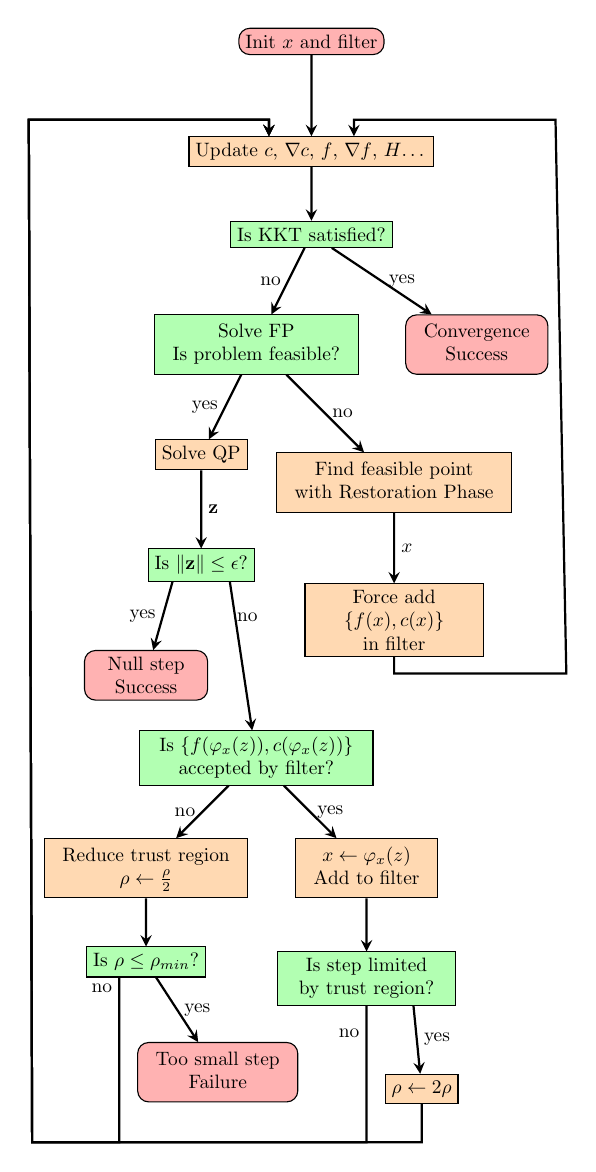
\begin{tikzpicture}[node distance=2cm, scale=0.7, every node/.style={transform shape}]

\node (init) [startstop] {Init $x$ and filter};
\node (update) [process, below of=init] {Update $c$, $\nabla c$, $f$, $\nabla f$, $H$\ldots};
\node (KKT) [decision, below of=update, yshift=0.5cm] {Is KKT satisfied?};
\node (success) [startstop, below of=KKT, xshift=3cm] {\begin{tabular}{c}Convergence\\ Success\end{tabular}};
\node (FP) [decision, below of=KKT, xshift=-1cm] {\begin{tabular}{c}Solve FP\\ Is problem feasible?\end{tabular}};
\node (QP) [process, below of=FP, xshift=-1cm] {Solve QP};
\node (restoration) [process, below of=FP, xshift=25mm, yshift=-0.5cm] {\begin{tabular}{c}Find feasible point\\ with Restoration Phase\end{tabular}};
\node (forceAdd) [process, below of=restoration, text width=3cm, yshift=-0.5cm] {Force add $\{f(x),c(x)\}$ in filter};
\node (zeroStep) [decision, below of=QP] {Is $\|\mathbf{z}\| \leq \epsilon$?};
\node (success2) [startstop, below of=zeroStep, xshift=-1cm, text width=2cm] {Null step Success};
\node (filterTest) [decision, below of=zeroStep, text width=4cm, yshift=-1.5cm, xshift=1cm] {Is $\{f(\varphi_x(z)),c(\varphi_x(z))\}$ accepted by filter?};
\node (reduceTR) [process, below of=filterTest, xshift=-2cm] {\begin{tabular}{c}Reduce trust region\\ $\rho\leftarrow\frac{\rho}{2}$\end{tabular}};
\node (smallStepTest) [decision, below of=reduceTR, yshift=3mm] {Is $\rho \leq \rho_{min}$?};
\node (fail) [startstop, below of=smallStepTest, xshift=13mm, yshift=0mm] {\begin{tabular}{c}Too small step\\
Failure\end{tabular}};
\node (addToFilter) [process, below of=filterTest, xshift=2cm] {\begin{tabular}{c}$x\leftarrow\varphi_x(z)$\\Add to filter\end{tabular}};
\node (limitedStep) [decision, below of=addToFilter, xshift=0mm, yshift=0mm, text width=30mm] {Is step limited by trust region?};
\node (increaseTR) [process, below of=limitedStep, xshift=1cm] {$\rho\leftarrow 2 \rho$};

\draw [arrow] (init) -- (update);
\draw [arrow] (update) -- (KKT);
\draw [arrow] (KKT) -- node[anchor=east] {no} (FP);
\draw [arrow] (KKT) -- node[anchor=west] {yes} (success);
\draw [arrow] (FP) -- node[anchor=east] {yes} (QP);
\draw [arrow] (FP) -- node[anchor=west] {no} (restoration);
\draw [arrow] (restoration) -- node[anchor=west] {$x$} (forceAdd);
\draw [arrow] (QP) -- node[anchor=west] {$\bf z$} (zeroStep);
\draw [arrow] (zeroStep.210) -- node[anchor=east] {yes} (success2);
\draw [arrow] (zeroStep.330) -- node[anchor=west, shift={(-2mm,7mm)}] {no} (filterTest);
\draw [arrow] (filterTest) -- node[anchor=east] {no} (reduceTR);
\draw [arrow] (filterTest) -- node[anchor=west] {yes}  (addToFilter);
\draw [arrow] (reduceTR) -- (smallStepTest);
\draw [arrow] (addToFilter) -- (limitedStep);
\draw [arrow] (smallStepTest) -- node[anchor=west] {yes} (fail);
\draw [arrow] (limitedStep.330) -- node[anchor=west] {yes} (increaseTR);
\draw [arrow] (forceAdd) |-([shift={(15mm,-3mm)}]forceAdd.south east)-- ([shift={(22mm,3mm)}]update.north east)-|(update.20);
\draw [arrow] (increaseTR) |-([shift={(-64mm,-7mm)}]increaseTR.south west)-- ([shift={(-29mm,3mm)}]update.north west)-| (update.160);
\draw [arrow] (limitedStep)node[anchor=east, yshift=-10mm] {no} |-([shift={(-64mm,-7mm)}]increaseTR.south west)-- ([shift={(-29mm,3mm)}]update.north west)-| (update.160);
\draw [arrow] (smallStepTest.210) node[anchor=east, yshift=-2mm] {no}|-([shift={(-64mm,-7mm)}]increaseTR.south west)-- ([shift={(-29mm,3mm)}]update.north west)-| (update.160);

\end{tikzpicture}
}

  \caption{Main SQP Loop}
\label{fig:main_sqp_loop}
\end{figure}

\begin{figure}[H]
  \begin{minipage}{.5\textwidth}
    \centering
    
\tikzstyle{startstop} = [rectangle, rounded corners, text centered, draw=black, fill=red!30]
\tikzstyle{process} = [rectangle, text centered, draw=black, fill=orange!30]
\tikzstyle{decision} = [rectangle, text centered, draw=black, fill=green!30]
\tikzstyle{arrow} = [thick,->,>=stealth]

\framebox{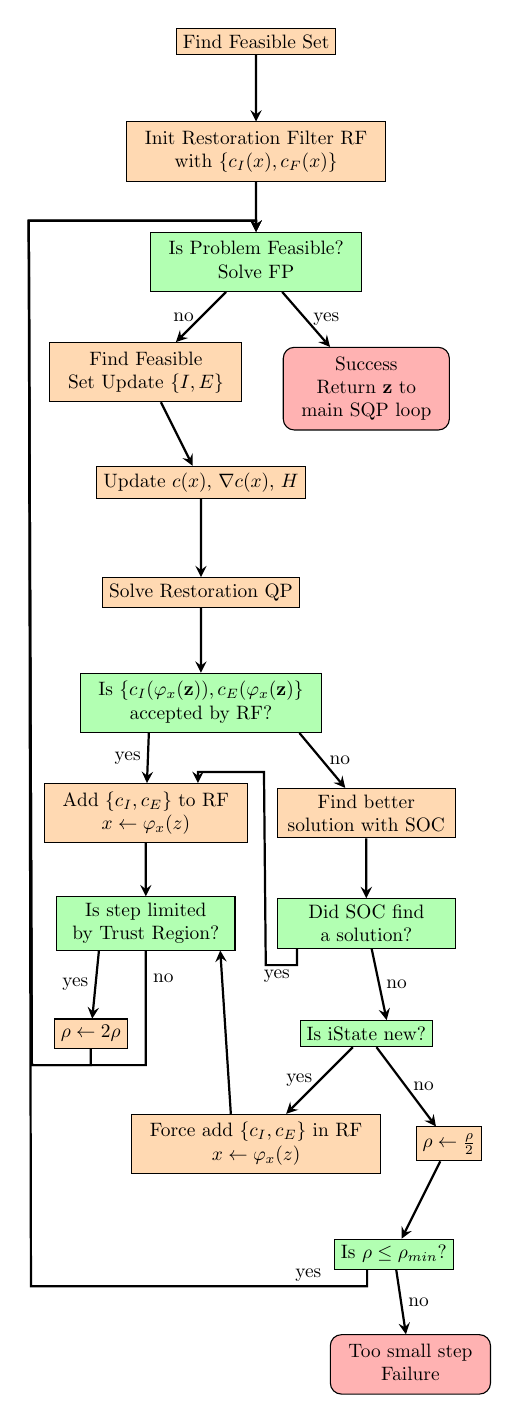
\begin{tikzpicture}[node distance=2cm, scale=0.7, every node/.style={transform shape}]

\node (feasibleSet) [process] {Find Feasible Set};
\node (init) [process, below of=feasibleSet] {\begin{tabular}{c}Init Restoration Filter RF\\with $\{c_I(x),c_F(x)\}$\end{tabular}};
\node (feasibleTest) [decision, below of=init] {\begin{tabular}{c}Is Problem Feasible?\\Solve FP\end{tabular}};
\node (success) [startstop, below of=feasibleTest, xshift=2cm, yshift=-3mm] {\begin{tabular}{c}Success\\Return $\bf z$ to\\main SQP loop\end{tabular} };
\node (findFeasibleSet) [process, below of=feasibleTest, xshift=-2cm] {\begin{tabular}{c} Find Feasible\\ Set Update $\{I,E\}$ \end{tabular}};
\node (update) [process, below of=findFeasibleSet, xshift=1cm] {Update $c(x)$, $\nabla c(x)$, $H$};
\node (QP) [process, below of=update] {Solve Restoration QP};
\node (filterTest) [decision, below of=QP] {\begin{tabular}{c}Is $\{c_I(\varphi_x(\mathbf{z})),c_E(\varphi_x(\mathbf{z})\}$\\accepted by RF?\end{tabular}};
\node (addFilter) [process, below of=filterTest, xshift=-1cm] {\begin{tabular}{c} Add $\{c_I,c_E\}$ to RF\\ $x\leftarrow\varphi_x(z)$\end{tabular}};
\node (stepLimited) [decision, below of=addFilter, text width=3cm] {Is step limited by Trust Region?};
\node (increaseTR) [process, below of=stepLimited, xshift=-1cm] {$\rho\leftarrow 2\rho$};
\node (SOC) [process, below of=filterTest, text width=3cm, xshift=3cm] {Find better solution with SOC};
\node (findSOC) [decision, below of=SOC, text width=3cm] {Did SOC find a solution?};
\node (iStateTest) [decision, below of=findSOC] {Is iState new?};
\node (forceAdd) [process, below of=iStateTest, xshift=-2cm] {\begin{tabular}{c} Force add $\{c_I,c_E\}$ in RF\\ $x\leftarrow\varphi_x(z)$\end{tabular}};
\node (reduceTR) [process, below of=iStateTest, xshift=1.5cm] {$\rho\leftarrow\frac{\rho}{2}$};
\node (tooSmallStep) [decision, below of=reduceTR, xshift=-1cm] {Is $\rho\leq\rho_{min}$?};
\node (fail) [startstop, below of=tooSmallStep, xshift=3mm] {\begin{tabular}{c}Too small step\\
Failure\end{tabular}};

\draw [arrow] (feasibleSet) -- (init);
\draw [arrow] (init) -- (feasibleTest);
\draw [arrow] (feasibleTest) -- node[anchor=west] {yes} (success);
\draw [arrow] (feasibleTest) -- node[anchor=east] {no} (findFeasibleSet);
\draw [arrow] (findFeasibleSet) -- (update);
\draw [arrow] (update) -- (QP);
\draw [arrow] (QP) -- (filterTest);
\draw [arrow] (filterTest.210) -- node[anchor=east] {yes} (addFilter);
\draw [arrow] (filterTest.343) -- node[anchor=west] {no} (SOC);
\draw [arrow] (addFilter) -- (stepLimited);
\draw [arrow] (stepLimited.210) -- node[anchor=east] {yes} (increaseTR);
\draw [arrow] (SOC) -- (findSOC);
\draw [arrow] (findSOC) [xshift=3cm]-- node[anchor=west] {no} (iStateTest);
\draw [arrow] (iStateTest) -- node[anchor=east] {yes} (forceAdd);
\draw [arrow] (iStateTest) -- node[anchor=west] {no} (reduceTR);
\draw [arrow] (reduceTR) -- (tooSmallStep);
\draw [arrow] (tooSmallStep) -- node[anchor=west] {no} (fail);
\draw [arrow] (forceAdd.130) -- (stepLimited.340);

\draw [arrow] (increaseTR) |-([shift={(-4mm,-3mm)}]increaseTR.south west)-- ([shift={(-22mm,2mm)}]feasibleTest.north west)-| (feasibleTest);
\draw [arrow] (stepLimited)  node[anchor=west, yshift=-1cm] {no} |-([shift={(-4mm,-3mm)}]increaseTR.south west)-- ([shift={(-22mm,2mm)}]feasibleTest.north west)-| (feasibleTest);
\draw [arrow] (tooSmallStep.210) node[anchor=east, shift={(-7mm,-1mm)}] {yes} |-([shift={(-55mm,-3mm)}]tooSmallStep.south west)-- ([shift={(-22mm,2mm)}]feasibleTest.north west)-| (feasibleTest);
\draw [arrow] (findSOC.200)  node[anchor=east, yshift=-5mm] {yes} |-([shift={(-2mm,-3mm)}]findSOC.south west) [xshift=1cm]-- ([shift={(3mm,2mm)}]addFilter.north east)-| (addFilter.30);

\end{tikzpicture}
}

    \caption{Restoration Loop}
\label{fig:restoration_loop}
  \end{minipage}%
  \begin{minipage}{.5\textwidth}
    \centering
    
\tikzstyle{startstop} = [rectangle, rounded corners, text centered, draw=black, fill=red!30]
\tikzstyle{process} = [rectangle, text centered, draw=black, fill=orange!30]
\tikzstyle{decision} = [rectangle, text centered, draw=black, fill=green!30]
\tikzstyle{arrow} = [thick,->,>=stealth]

\framebox{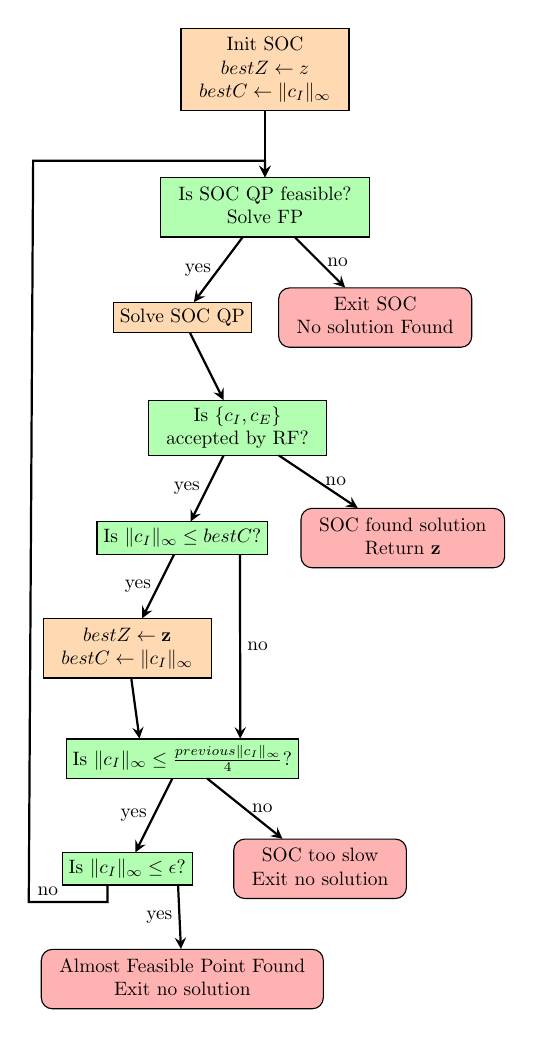
\begin{tikzpicture}[node distance=2cm, scale=0.7, every node/.style={transform shape}]

\node (init) [process] {\begin{tabular}{c}Init SOC\\ $bestZ\leftarrow z$\\ $bestC\leftarrow\|c_I\|_\infty$\end{tabular}};
\node (FPTest) [decision, below of=init, yshift=-5mm] {\begin{tabular}{c}Is SOC QP feasible?\\Solve FP\end{tabular}};
\node (noSolution) [startstop, below of=FPTest, xshift=2cm] {\begin{tabular}{c}Exit SOC\\No solution Found\end{tabular}};
\node (QP) [process, below of=FPTest, xshift=-15mm] {Solve SOC QP};
\node (filterTest) [decision, below of=QP, text width=3cm, xshift=10mm] {Is $\{c_I,c_E\}$ accepted by RF?};
\node (success) [startstop, below of=filterTest, xshift=30mm] {\begin{tabular}{c}SOC found solution\\Return $\bf z$\end{tabular}};
\node (betterViolTest) [decision, below of=filterTest, xshift=-10mm] {Is $\|c_I\|_\infty\leq bestC$?};
\node (updateBest) [process, below of=betterViolTest, xshift=-10mm] {\begin{tabular}{c}$bestZ\leftarrow \bf z$  \\ $bestC\leftarrow\|c_I\|_\infty$ \end{tabular}};
\node (tooSlowTest) [decision, below of=updateBest, xshift=10mm] {Is $\|c_I\|_\infty\leq \frac{previous \|c_I\|_\infty}{4}$?};
\node (almostFeasibleTest) [decision, below of=tooSlowTest, xshift=-10mm] {Is $\|c_I\|_\infty\leq\epsilon$?};
\node (tooSlowFail) [startstop, below of=tooSlowTest, xshift=25mm] {\begin{tabular}{c}SOC too slow\\Exit no solution\end{tabular}};
\node (almostFeasible) [startstop, below of=almostFeasibleTest, xshift=10mm] {\begin{tabular}{c}Almost Feasible Point Found\\Exit no solution\end{tabular} };

\draw [arrow] (init) -- (FPTest);
\draw [arrow] (FPTest) -- node[anchor=west] {no}  (noSolution);
\draw [arrow] (FPTest) -- node[anchor=east] {yes} (QP);
\draw [arrow] (QP) -- (filterTest);
\draw [arrow] (filterTest) -- node[anchor=west] {no} (success);
\draw [arrow] (filterTest) -- node[anchor=east] {yes}(betterViolTest);
\draw [arrow] (betterViolTest) -- node[anchor=east] {yes} (updateBest);
\draw [arrow] (betterViolTest.344) -- node[anchor=west] {no}(tooSlowTest.19);
\draw [arrow] (updateBest) -- (tooSlowTest.155);
\draw [arrow] (tooSlowTest) -- node[anchor=west] {no}(tooSlowFail);
\draw [arrow] (tooSlowTest) -- node[anchor=east] {yes}(almostFeasibleTest);
\draw [arrow] (almostFeasibleTest.342) --node[anchor=east] {yes} (almostFeasible);
\draw [arrow] (almostFeasibleTest.220) node[anchor=west, shift={(-14mm,-1mm)}] {no}|-([shift={(-6mm,-3mm)}]almostFeasibleTest.south west)-- ([shift={(-23mm,3mm)}]FPTest.north west)-| (FPTest);

\end{tikzpicture}
}

    \caption{Second Order Correction}
\label{fig:second_order_correction}
  \end{minipage}%
\end{figure}

\section{Conclusion}
\label{sec:conclusion}

In this chapter, we presented the principle of nonlinear optimization on non-Euclidean manifolds, and detailed the choices we made to implement an SQP algorithm that solves those problems efficiently.
In addition to being used in our posture generation problems, {\tt PGSolver} has been used successfully in inertia identification problems as presented in~\cite{traversaro:iros:2016}.
In the next section, we will focus on the formulation of optimization problems for posture generation.

%}}}

